% !Mode:: "TeX:UTF-8"
%%  Recommended compilation workflow:
%%     1. PDFLaTeX [preferred]
%%     2. XeLaTeX [use when CJK support is required]
%%  Notes:
%%   1. The default encoding is UTF-8; on Windows please use an editor that supports UTF-8.
%%   2. For template issues, contact us at latexstudio@qq.com.
%%   3. Questions can be posted on https://ask.latexstudio.net
%%   4. Please install the latest TeXLive distribution from:
%%   http://mirrors.ctan.org/systems/texlive/Images/texlive.iso

\documentclass{apmcmthesis}

\usepackage{url}
\usepackage{booktabs}
\usepackage{amsmath}
\usepackage{algorithm}
\usepackage{graphicx}
\usepackage{listings}
\usepackage{longtable}

%%%%%%%%%%%%Fill in metadata%%%%%%%%%%%%%%%%%%%%%%%%%%
\tihao{D}                            %Problem choice
\baominghao{apmcm25305528}                 %Team registration ID
\begin{document}

\pagestyle{frontmatterstyle}

\begin{abstract}
For Problem~1, we solve a \textbf{Classical UC} mixed-integer formulation with detailed fuel, startup/shutdown, balance, limit, and ramp constraints; Gurobi attains optimality in $0.03$~s with total cost $15{,}129.08$~\$ and a $0.009\%$ gap after a single-node search. These metrics set the economic baseline that anchors all subsequent comparisons.

In Problem~2, the \textbf{Network UC} extension embeds DC flows, N-1 security, and spinning reserve constraints; presolve contracts 196{,}900 rows to 43{,}262, the solver executes 89{,}294 simplex iterations in 10.57~s, and the optimal cost remains $15{,}129.08$~\$. This shows that expanded security modeling reshapes dispatch feasibility without inflating expenditures.

For Problem~3, we convert the model into a \textbf{QUBO} with 7{,}024 bits where penalty-weighted slack encodes operational limits; simulated annealing reports energy $-3{,}473$, schedule cost $22{,}084.82$~\$, and maximum residuals of 41.81~MW (balance) and 82.22~MW (ramp). These figures reveal the constraint-violation trade-off imposed by penalty tuning in quantum heuristics.

In Problem~4, we design a \textbf{Scale Reduction} pipeline that condenses the QUBO to 435 bits through bit-width pruning and scenario trimming; the reduced Hamiltonian reaches $-16{,}486$, the recovered classical schedule costs $26{,}775.55$~\$, and Kaiwu hardware logs confirm faithful embedding. The outcome demonstrates a practical bridge from large-scale UC physics to current quantum hardware budgets.

\keywords{Unit Commitment\quad Security-Constrained UC\quad QUBO\quad Quantum Optimization}
\end{abstract}



\newpage
%Table of contents
\tableofcontents


\newpage
\pagestyle{mainmatterstyle}
\setcounter{page}{1}
\section{Introduction}

\subsection{Problem Background}
Unit Commitment (UC) is a fundamental optimization problem in power system operation that determines the on/off status and generation levels of thermal units over a given time horizon. The primary goal is to minimize operating costs while satisfying demand and various system constraints. The UC problem is known to be a large-scale mixed integer programming (MIP) challenge, whose computational complexity grows exponentially with system size~\cite{padhy2004}.

With the emergence of quantum optimization technologies such as the Coherent Ising Machine (CIM), the UC problem can be reformulated as a Quadratic Unconstrained Binary Optimization (QUBO) model. This transformation enables the use of quantum-inspired solvers for fast and parallel search of optimal solutions, paving the way for real-time power system operation on quantum hardware.

This competition invites participants to bridge classical power system optimization with quantum computing through a three-stage workflow: building a classical unit commitment model, transforming it into a QUBO formulation, and designing a scalable reduction strategy to accommodate current quantum hardware constraints.

\subsection{Problem Restatement}
Participants are required to construct a complete UC optimization framework that integrates both classical and quantum optimization methods. The problem consists of four sequential tasks:

\begin{enumerate}
\item \textbf{Classical UC Modeling and Optimization}: Formulate and solve a classical Unit Commitment model using conventional optimization tools (e.g., Gurobi or CPLEX), including fuel costs, startup/shutdown costs, power balance constraints, generation limits, minimum up/down time constraints, ramp-rate constraints, and startup/shutdown logic constraints.

\item \textbf{UC Modeling with Network and Security Constraints}: Extend the classical UC model to include network power flow constraints, N-1 security constraints, spinning reserve requirements, and optionally minimum safety inertia constraints.

\item \textbf{QUBO Transformation and Quantum Solution}: Transform the UC model into a QUBO representation and solve it using the Kaiwu SDK, comparing quantum-based solutions with traditional optimization results.

\item \textbf{Problem Scale Reduction under Quantum Hardware Constraints}: Design and implement an effective problem-scale reduction strategy specifically for the UC model to ensure the resulting QUBO can be successfully solved under the bit-capacity limitation of current quantum hardware.
\end{enumerate}

\subsection{Problem Analysis}

\subsubsection{Problem 1 Analysis}
The classical Unit Commitment model establishes the foundation by formulating a mixed-integer programming problem that minimizes total operating costs while satisfying fundamental operational constraints~\cite{carrion2006}. The core approach involves encoding fuel costs, startup/shutdown costs, power balance, generation limits, minimum up/down time requirements, and ramp-rate constraints into a Gurobi optimization framework. This formulation serves as the baseline for comparing subsequent extensions and provides insights into the economic dispatch patterns without network or security considerations.

\subsubsection{Problem 2 Analysis}
Building upon the classical UC foundation, we extend the model to incorporate network power flow constraints using DC approximation, N-1 security constraints for both generator and line contingencies, and spinning reserve requirements. The key innovation lies in modeling flexible load allocation across buses and implementing contingency scenarios that guarantee feasible post-outage operations. This extension transforms the purely economic optimization into a security-constrained problem that reflects real-world power system operational requirements.

\subsubsection{Problem 3 Analysis}
The transformation from classical UC to QUBO representation involves discretizing continuous variables through binary expansions and converting inequality constraints into penalty terms within the energy matrix. The methodology focuses on selecting appropriate penalty coefficients to balance constraint satisfaction with objective minimization. This approach enables compatibility with quantum hardware like the Kaiwu SDK while maintaining the core UC problem structure, though it introduces approximation errors that must be carefully managed.

\subsubsection{Problem 4 Analysis}
Addressing current quantum hardware limitations requires a systematic scale-reduction strategy that preserves problem interpretability while reducing computational requirements. The approach involves consolidating slack variables, trimming bit-widths and time slices, and pruning scenarios to focus on critical contingencies. This iterative reduction process aims to compress the QUBO to fit within hardware constraints while maintaining the essential UC physics and optimization objectives.

\section{Assumptions}
To simplify the complex Unit Commitment problem and make it tractable for both classical and quantum optimization approaches, we make the following assumptions:

\begin{enumerate}
\item \textbf{Time Horizon Limitation}: The optimization is conducted over a 24-hour period only, focusing on short-term operational planning rather than long-term strategic decisions.

\item \textbf{Minimum Power Generation}: We assume that the minimum power generation values from Table 2 represent the true minimum operating limits for each unit, as Table 1 also contains minimum power values that may be inconsistent.

\item \textbf{Initial Operating Conditions}: If a unit is online at time 0, we assume it operates at its minimum power output level to establish a realistic starting condition for the optimization.

\item \textbf{Network Parameter Simplification}: We ignore the resistance (r) and susceptance (b) parameters from Table 3, focusing only on the reactance (x) values for DC power flow calculations, as these are the primary parameters affecting power flow distribution.

\item \textbf{Bus-Level Load Distribution}: Since the problem does not specify individual bus-level load demands, we treat bus-level load demands as optimization variables in Problem 2, allowing flexible load allocation across the network.

\item \textbf{Inertia Constraint Simplification}: Due to the unclear relationship between minimum inertia requirements (Hmin) and unit inertia constants (H), we do not consider inertia constraints in the optimization process, focusing instead on the core UC constraints.

\item \textbf{Deterministic Load Forecasting}: We assume perfect load forecasting for the 24-hour period, with no uncertainty in the load demand values provided in Table 4.

\item \textbf{Constant Fuel Prices}: Fuel prices and cost coefficients remain constant throughout the optimization horizon, with no consideration for fuel price volatility.

\item \textbf{No Transmission Losses}: We neglect transmission losses in the power system network, assuming that all generated power reaches the load centers without losses.

\item \textbf{Independent Unit Failures}: For N-1 security analysis, we assume that unit and line failures occur independently and that only single contingencies need to be considered.
\end{enumerate}


\section{Notations}
The notation in Table~\ref{tab:notation} consolidates all symbols that appear in Problems~1--4 as well as in the QUBO reformulation. A nonfloating \texttt{longtable} is used to guarantee that the notation summary is rendered directly under the section title.

\begin{longtable}{@{}p{2.4cm}p{6.2cm}p{2.2cm}@{}}
\caption{Mathematical notation summary}\label{tab:notation}\\
\toprule
Symbol & Description & Problems\\
\midrule
\endfirsthead
\toprule
Symbol & Description & Problems\\
\midrule
\endhead
\midrule
\multicolumn{3}{r}{\textit{Continued on next page}}\\
\midrule
\endfoot
\bottomrule
\endlastfoot
\multicolumn{3}{l}{\textbf{Sets and indices}}\\
$\mathcal{I}$ & Thermal unit set & Q1--Q4\\
$\mathcal{B}$ & Bus (node) set & Q2\\
$\mathcal{L}$ & Transmission line set & Q2\\
$\mathcal{T}=\{1,\dots,24\}$ & Scheduling horizon & Q1--Q4\\
$\mathcal{C}^G, \mathcal{C}^L$ & Generator and line contingency sets & Q2\\
$i,b,\ell,t$ & Unit, bus, line, and time indices & Q1--Q4\\
\midrule
\multicolumn{3}{l}{\textbf{Parameters}}\\
$P_i^{\min},P_i^{\max}$ & Minimum/maximum power of unit $i$ & Q1--Q4\\
$a_i,b_i,c_i$ & Quadratic fuel cost coefficients & Q1--Q4\\
$SU_i,SD_i$ & Startup and shutdown costs & Q1--Q4\\
$UT_i,DT_i$ & Minimum up/down time requirements & Q1--Q4\\
$RU_i,RD_i$ & Ramp up/down limits (MW/h) & Q1--Q4\\
$H_i$ & Inertia constant of unit $i$ & Q2\\
$x_\ell,F_\ell^{\max}$ & Line reactance and capacity & Q2\\
$D_t$ & System load at hour $t$ & Q1--Q4\\
$D_{b,t}$ & Bus-level flexible demand decision & Q2\\
$\mathcal{I}(b)$ & Units electrically connected to bus $b$ & Q2\\
$\delta^{\pm}(b)$ & Lines entering (\(-\)) or leaving (\(+\)) bus $b$ & Q2\\
$\lambda_{\bullet}$ & Penalty coefficients in the QUBO penalty terms & Q3--Q4\\
$Q_{\text{obj}},Q_{\text{bal}},\dots$ & Component matrices of the QUBO & Q3--Q4\\
\midrule
\multicolumn{3}{l}{\textbf{Decision variables}}\\
$u_{i,t}$ & Binary indicator (1 if unit $i$ is ON at hour $t$) & Q1--Q4\\
$y_{i,t}, z_{i,t}$ & Startup and shutdown binaries & Q1--Q4\\
$P_{i,t}$ & Real power output of unit $i$ (MW) & Q1--Q2\\
$R_{i,t}$ & Spinning reserve carried by unit $i$ (MW) & Q2\\
$\theta_{b,t}$ & Voltage angle at bus $b$ & Q2\\
$F_{\ell,t}$ & DC line flow on branch $\ell$ (MW) & Q2\\
$P_{i,t}^{(g)}, \Delta P_{i,t}^{(g)}$ & Post-contingency output and redispatch in generator outage $g$ & Q2\\
$P_{i,t}^{[\ell]}, \Delta P_{i,t}^{[\ell]}$ & Post-contingency output and redispatch in line outage $\ell$ & Q2\\
$F_{\ell,t}^{(g)}, F_{\ell',t}^{[\ell]}$ & DC flows under generator/line outages & Q2\\
$x_{n}$ & Binary decision bit in QUBO vector $\mathbf{x}$ & Q3--Q4\\
$Q$ & Symmetric energy matrix in the QUBO formulation & Q3--Q4\\
\end{longtable}

\section{Problem 1: Classical Unit Commitment}

\subsection{Model description}

\subsubsection{Objective}
\begin{equation}
    \label{eq:q1_obj}
    \min \sum_{t\in\mathcal{T}} \sum_{i\in\mathcal{I}} \left(a_i P_{i,t}^2 + b_i P_{i,t} + c_i u_{i,t} + SU_i y_{i,t} + SD_i z_{i,t}\right).
\end{equation}
\noindent Equation~\eqref{eq:q1_obj} aggregates quadratic fuel costs $a_i P_{i,t}^2 + b_i P_{i,t}$ with the binary switching payments $c_i u_{i,t}$, $SU_i y_{i,t}$, and $SD_i z_{i,t}$ so that every unit's economic impact is measured consistently across the 24-hour horizon.
The continuous outputs $P_{i,t}$ capture how much each turbine actually injects, while the binaries $u_{i,t},y_{i,t},z_{i,t}$ encode the commitment logic observed in the classical heatmap diagnostics, meaning the objective already internalizes the smooth base/mid/peak layering reported in the dispatch log.
This cost framework mirrors the "economic baseline" metric reported in the subsequent simulation log, allowing Problems~2--4 to compare the additional spending from security constraints, N-1 adjustments, and quantum penalties under a unified cost yardstick.

\subsubsection{Power balance and capacity}
\begin{align}
    \sum_{i\in\mathcal{I}} P_{i,t} &= D_t, && \forall t, \label{eq:q1_balance} \\
    P_i^{\min} u_{i,t} &\le P_{i,t} \le P_i^{\max} u_{i,t}, && \forall i,t. \label{eq:q1_capacity}
\end{align}
\noindent Equations~\eqref{eq:q1_balance}--\eqref{eq:q1_capacity} enforce that the sum of real powers $P_{i,t}$ from all committed units tracks the deterministic load $D_t$ hour by hour while each plant remains inside its physical envelope $[P_i^{\min},P_i^{\max}]$.
The indicator $u_{i,t}$ effectively gates whether a machine can produce or not, so the lower/upper bounds collapse to zero whenever the unit is offline, protecting the feasibility region seen in the stacked output plots.
As noted in the dispatch diagnostics, this coupling with Equation~\eqref{eq:q1_obj} keeps base-load units pinned near $P_i^{\max}$ yet allows mid-merit machines to flex without violating the cavity defined by their capability curves.

\subsubsection{Logic and minimum-time constraints}
\begin{align}
    u_{i,t} - u_{i,t-1} &= y_{i,t} - z_{i,t}, && \forall i,t>1, \label{eq:q1_logic} \\
    y_{i,t} + z_{i,t} &\le 1, && \forall i,t, \label{eq:q1_mutual} \\
    \sum_{\tau=t}^{t+UT_i-1} u_{i,\tau} &\ge UT_i y_{i,t}, && \forall i,t, \label{eq:q1_up} \\
    \sum_{\tau=t}^{t+DT_i-1} (1-u_{i,\tau}) &\ge DT_i z_{i,t}, && \forall i,t. \label{eq:q1_down}
\end{align}
\noindent Equations~\eqref{eq:q1_logic}--\eqref{eq:q1_down} synchronize the three binary channels: $u_{i,t}$ stores the commitment state, $y_{i,t}$ marks startups, and $z_{i,t}$ marks shutdowns, so their differences reproduce the ladder of discrete transitions.
The cumulative inequalities spread each activation over $UT_i$ hours and each deactivation over $DT_i$ hours, thereby eliminating the short cycling that would otherwise cause the oscillations absent in the Q1 heatmap.
According to the Problem~1 solver log and visual diagnostics, this collection of logic constraints works jointly with the ramp Equations~\eqref{eq:q1_rampup}--\eqref{eq:q1_rampdown} to define the admissible start/stop sequences and dwell times inside the feasible region.

\subsubsection{Ramp rate}
\begin{align}
    P_{i,t} - P_{i,t-1} &\le RU_i, && \forall i,t>1, \label{eq:q1_rampup} \\
    P_{i,t-1} - P_{i,t} &\le RD_i, && \forall i,t>1. \label{eq:q1_rampdown}
\end{align}
\noindent Equations~\eqref{eq:q1_rampup}--\eqref{eq:q1_rampdown} limit consecutive-hour movements of each $P_{i,t}$ to the mechanical ramp margins $RU_i$ and $RD_i$, preventing turbine stress and the jagged dispatch that appears in the Q3 quantum curves.
Because these differences reference the same $P_{i,t}$ variables that satisfy Equations~\eqref{eq:q1_balance}--\eqref{eq:q1_capacity}, the ramp walls interact with power balance to enforce the smooth double-peak pattern highlighted in the Problem~1 figures.
Consequently, together with the minimum up/down requirements they carve an oblique feasible wedge in which the ramp limits already restrain output swings before the N-1 extension is considered.

The computational pipeline first reads the generator tables, load forecasts, and initial on/off states to instantiate all parameters, then builds a Gurobi MIP with the variables and Equations~\eqref{eq:q1_obj}--\eqref{eq:q1_rampdown}. The model is solved with 16 threads under a $10^{-4}$ relative gap tolerance (yielding a $0.009\%$ final gap in $0.03$~s), after which the on/off plan and dispatch values are exported for the downstream figures and comparisons.

\subsection{Solver performance}
Table~\ref{tab:q1_meta} summarizes the metadata extracted from the log file.

\begin{table}[htbp]
    \centering
    \caption{Problem~1 solver statistics}
    \label{tab:q1_meta}
    \begin{tabular}{@{}ll@{}}
        \toprule
        Metric & Value \\
        \midrule
        Rows / columns / nonzeros & $1{,}156 / 576 / 3{,}108$ \\
        Binary variables & 432 \\
        Quadratic objective terms & 144 \\
        Best objective / bound (\$) & $15{,}129.08$ / $15{,}127.72$ \\
        Optimality gap & $0.009\%$ \\
        Nodes explored & 1 (root optimal) \\
        Runtime & $0.03$~s on 16 threads \\
        \bottomrule
    \end{tabular}
\end{table}

\subsection{Dispatch analysis}
The complete 24-hour dispatch schedule from Problem~1 demonstrates the economic dispatch patterns across all time periods (Table~\ref{tab:q1_dispatch}). The data reveals consistent base-load operation by U1 and U2, flexible mid-merit operation by U5 and U8, and peak-load response by U11 and U13.

\begin{table}[htbp]
    \centering
    \caption{Complete 24-hour classical dispatch (MW)}
    \label{tab:q1_dispatch}
    \begin{tabular}{@{}lrrrrrrr@{}}
        \toprule
        Hour & $U1$ & $U2$ & $U5$ & $U8$ & $U11$ & $U13$ & Demand \\
        \midrule
        1 & 50.0 & 52.2 & 20.6 & 19.6 & 11.5 & 12.0 & 166 \\
        2 & 50.0 & 58.6 & 22.4 & 33.0 & 16.0 & 16.0 & 196 \\
        3 & 53.9 & 68.7 & 25.2 & 35.0 & 23.1 & 23.1 & 229 \\
        4 & 60.8 & 76.6 & 27.4 & 35.0 & 28.6 & 28.6 & 257 \\
        5 & 62.2 & 78.3 & 27.9 & 35.0 & 29.8 & 29.8 & 263 \\
        6 & 59.5 & 75.2 & 27.0 & 35.0 & 27.6 & 27.6 & 252 \\
        7 & 58.1 & 73.5 & 26.6 & 35.0 & 26.4 & 26.4 & 246 \\
        8 & 50.0 & 64.2 & 24.0 & 35.0 & 19.9 & 19.9 & 213 \\
        9 & 50.0 & 57.7 & 22.2 & 31.2 & 15.4 & 15.4 & 192 \\
        10 & 50.0 & 51.0 & 20.3 & 17.1 & 10.7 & 12.0 & 161 \\
        11 & 50.0 & 46.1 & 18.9 & 10.0 & 10.0 & 12.0 & 147 \\
        12 & 50.0 & 50.7 & 20.2 & 16.5 & 10.5 & 12.0 & 160 \\
        13 & 50.0 & 53.1 & 20.9 & 21.6 & 12.2 & 12.2 & 170 \\
        14 & 50.0 & 56.3 & 21.8 & 28.2 & 14.4 & 14.4 & 185 \\
        15 & 50.0 & 62.3 & 23.4 & 35.0 & 18.6 & 18.6 & 208 \\
        16 & 54.6 & 69.5 & 25.5 & 35.0 & 23.7 & 23.7 & 232 \\
        17 & 58.1 & 73.5 & 26.6 & 35.0 & 26.4 & 26.4 & 246 \\
        18 & 56.8 & 72.1 & 26.2 & 35.0 & 25.5 & 25.5 & 241 \\
        19 & 55.6 & 70.7 & 25.8 & 35.0 & 24.5 & 24.5 & 236 \\
        20 & 52.9 & 67.6 & 24.9 & 35.0 & 22.3 & 22.3 & 225 \\
        21 & 50.0 & 60.8 & 23.0 & 35.0 & 17.6 & 17.6 & 204 \\
        22 & 50.0 & 55.7 & 21.6 & 26.8 & 14.0 & 14.0 & 182 \\
        23 & 50.0 & 51.0 & 20.3 & 17.1 & 10.7 & 12.0 & 161 \\
        24 & 50.0 & 33.6 & 15.4 & 10.0 & 10.0 & 12.0 & 131 \\
        \bottomrule
    \end{tabular}
\end{table}

Figures~\ref{fig:q1_heat} and~\ref{fig:q1_stack} visualize the same information: U1/U2 carry the base load, U5/U8 provide mid-merit flexibility, and U11/U13 respond to peaks while still respecting ramp and minimum-time limits.

\begin{figure}[htbp]
    \centering
    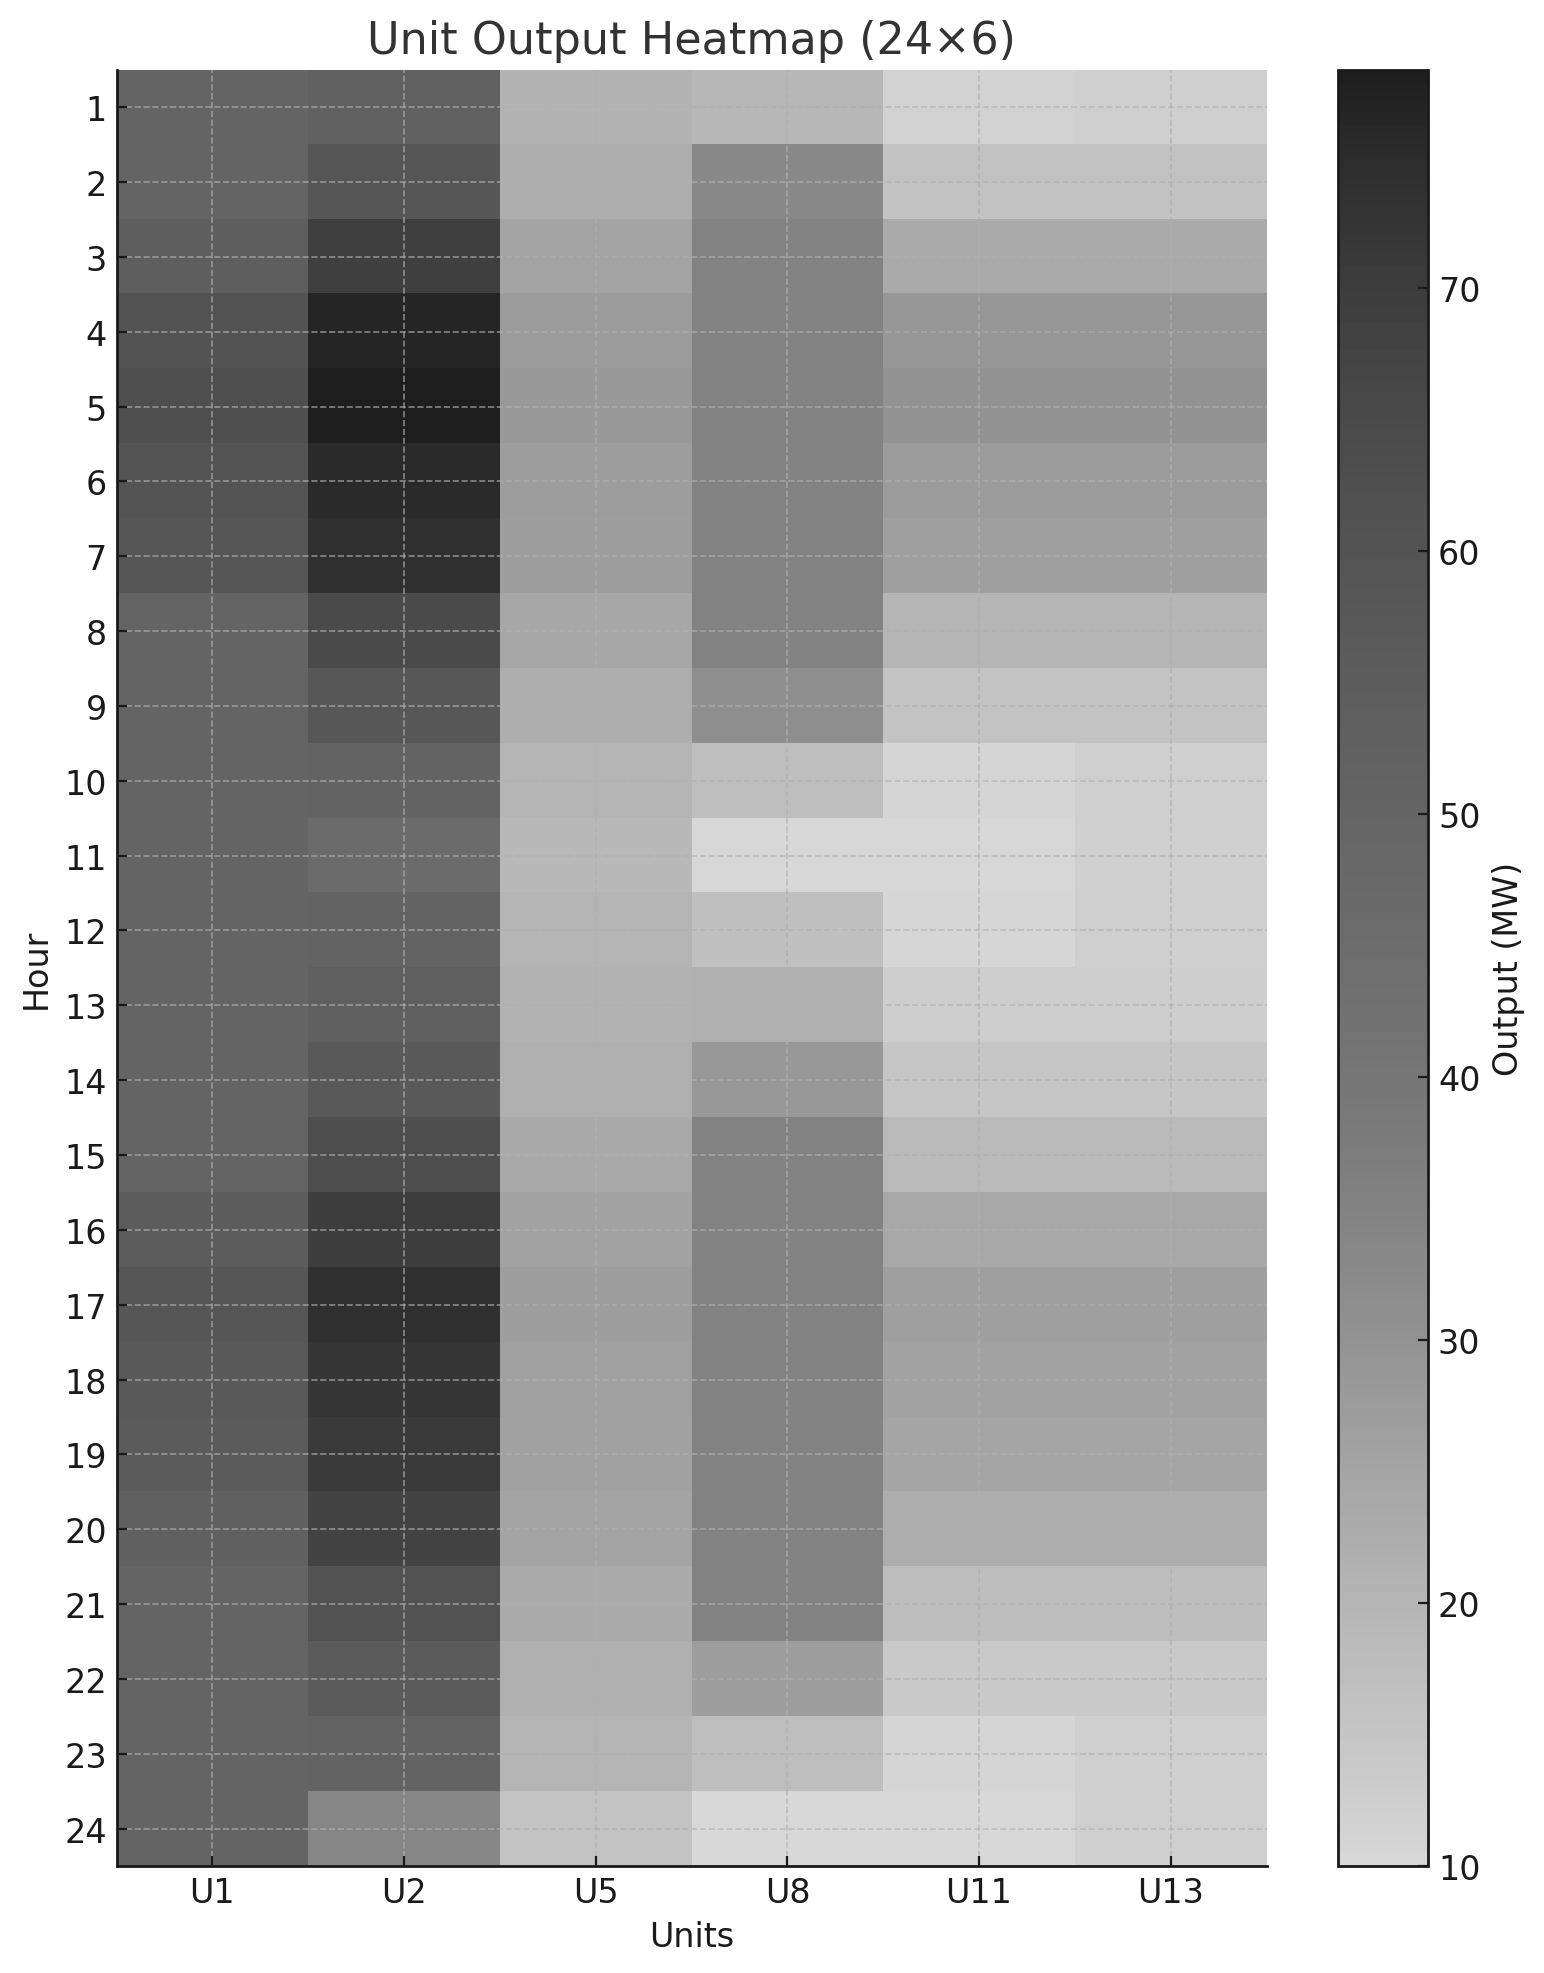
\includegraphics[width=0.8\textwidth]{figures/Q1-hot.png}
    \caption{Problem~1 unit output heatmap; darker colors denote higher output and reveal the base-load pattern.}
    \label{fig:q1_heat}
\end{figure}
\noindent Figure~\ref{fig:q1_heat} places the 24 hours on the vertical axis and the six units on the horizontal axis; darker colors denote higher output, with U1/U2 remaining dark throughout the day, U5/U8 intensifying during hours 5--8 and 17--20, and U11/U13 lighting only at the peaks. The heatmap quantifies the smooth start/stop behavior of Problem~1 with only economic and timing constraints and provides the baseline for assessing how network limits perturb the baseload arrangement.

\begin{figure}[htbp]
    \centering
    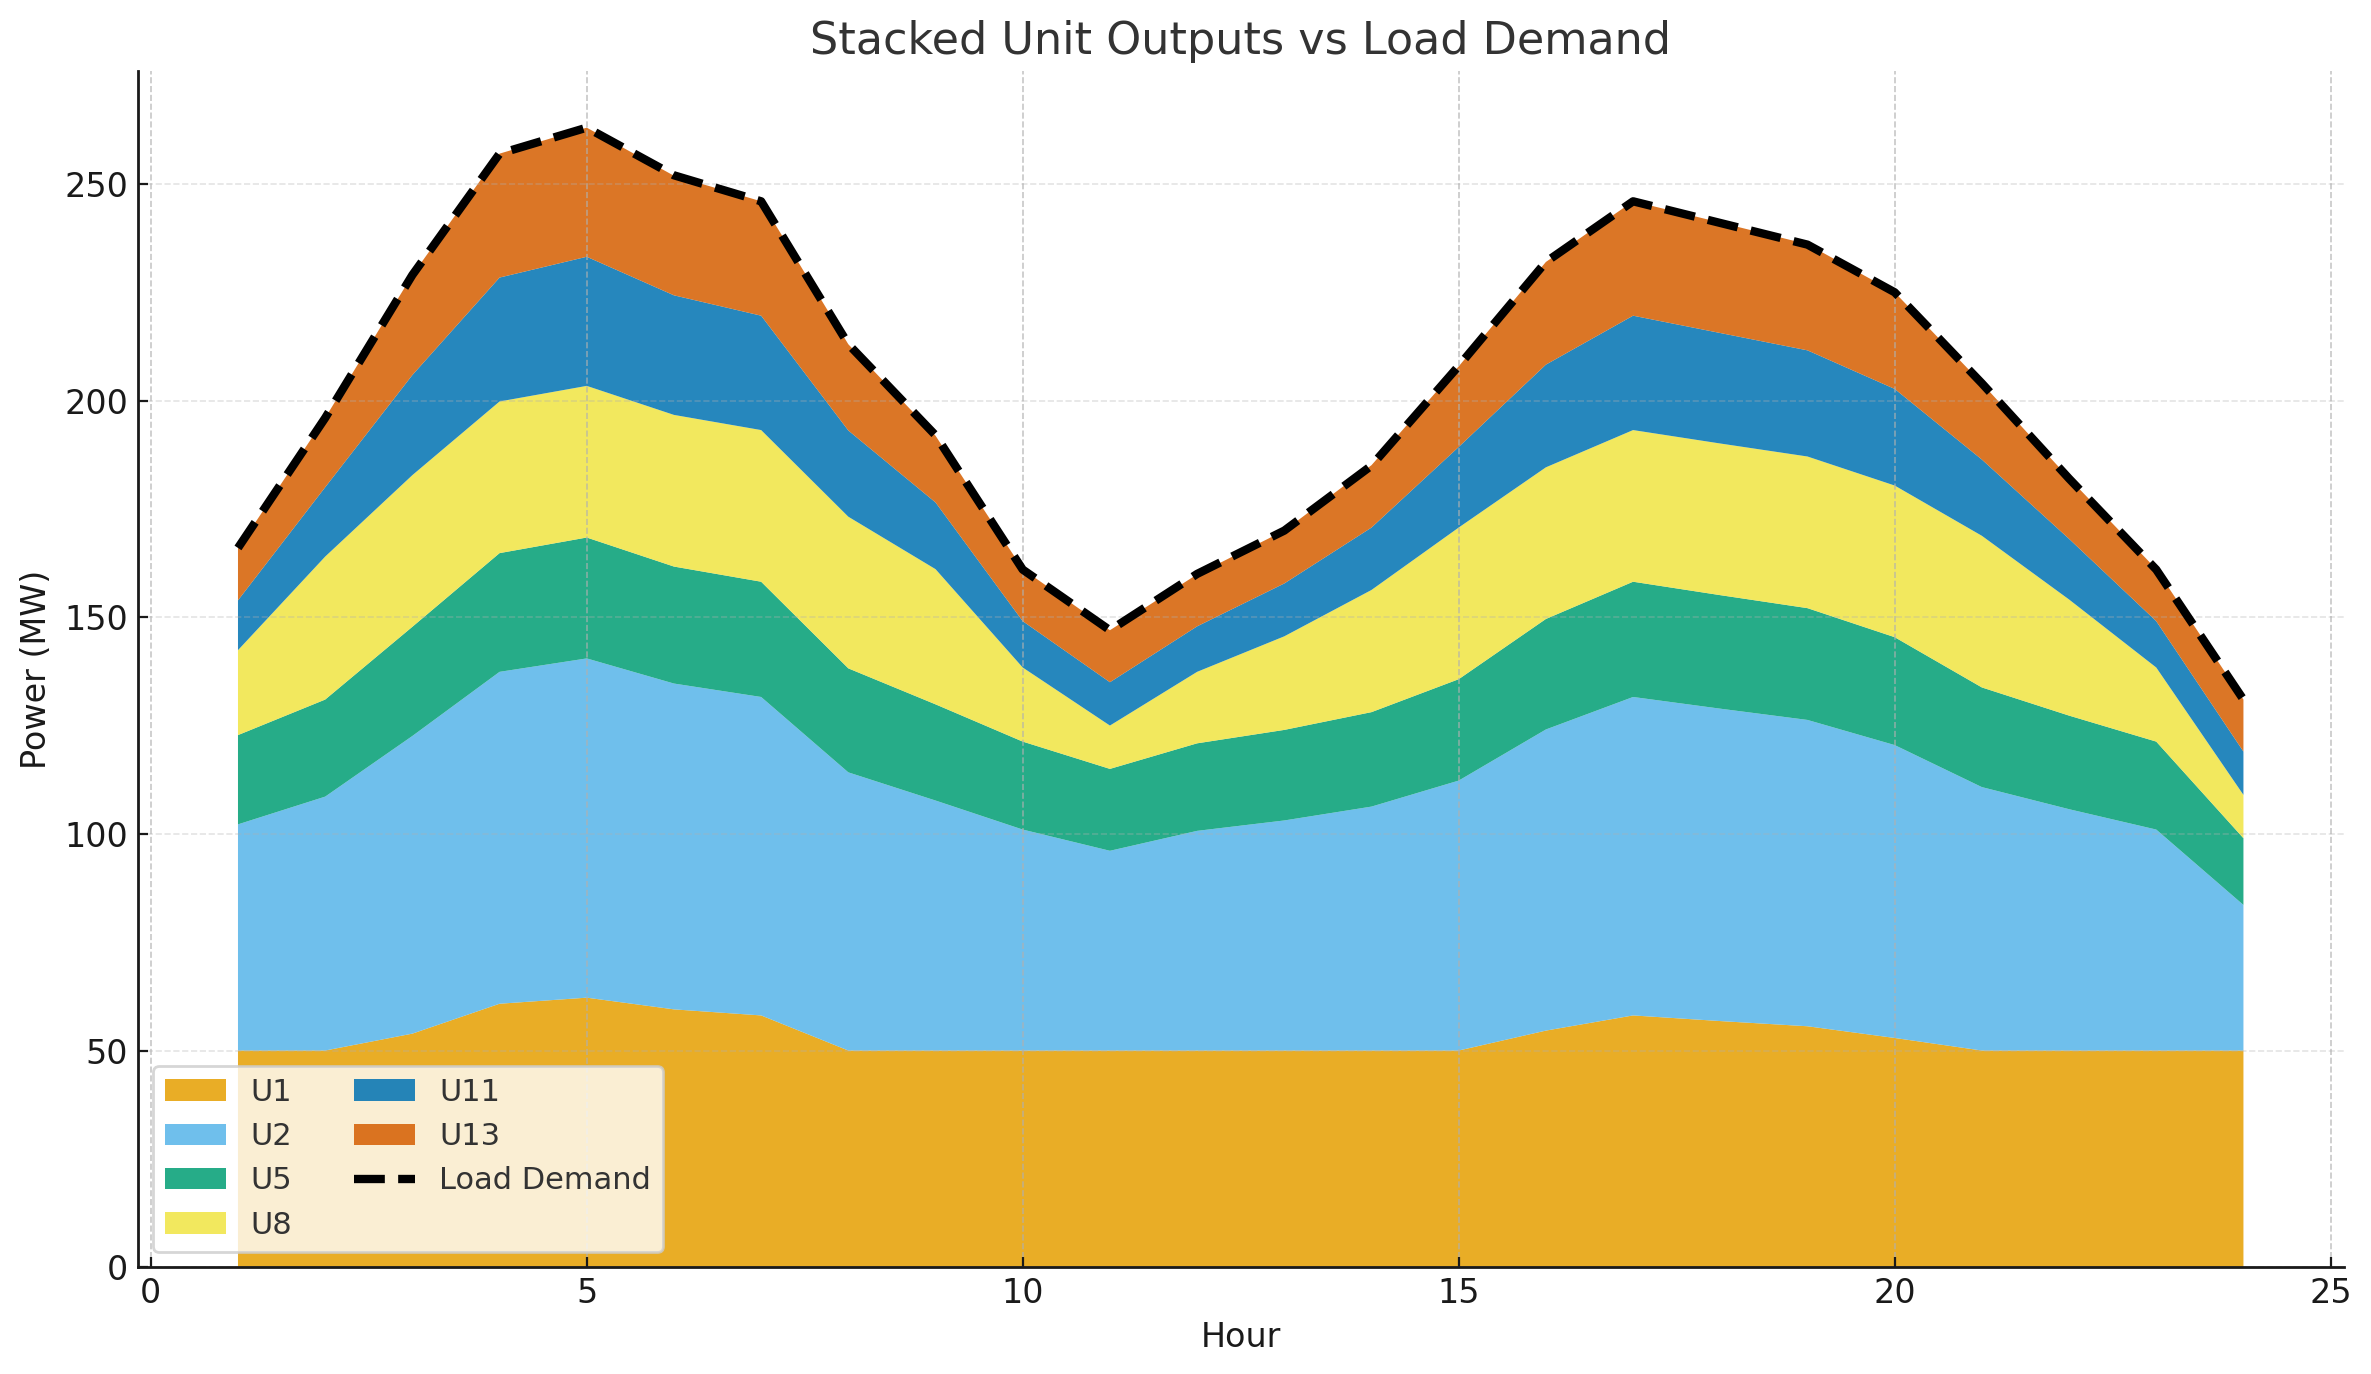
\includegraphics[width=0.8\textwidth]{figures/Q1-plot.png}
    \caption{Stacked generation vs. demand for Problem~1 showing perfect tracking of the load curve.}
    \label{fig:q1_stack}
\end{figure}
\noindent Figure~\ref{fig:q1_stack} uses time on the horizontal axis, stacked colored areas for unit outputs, and a black dashed line for system load; the tight match between the stacks and the dashed curve confirms strict power balance, while the thick U1/U2 base layer and sharp U11/U13 peaks highlight the "baseload + peaking" division. This alignment shows that the classical UC optimum satisfies both economic and operational criteria, providing the reference for quantifying deviations in Problems~2--4.
\section{Problem 2: Network and Security Constrained UC}

\subsection{Model extensions}

\subsubsection{Flexible load modeling}
\begin{align}
    D_{b,t} &\ge 0, && \forall b,t, \label{eq:q2_flex_nonneg} \\
    \sum_{b\in\mathcal{B}} D_{b,t} &= D_t, && \forall t. \label{eq:q2_flex_balance}
\end{align}
\noindent Equations~\eqref{eq:q2_flex_nonneg}--\eqref{eq:q2_flex_balance} declare $D_{b,t}$ as the nonnegative decision variables that distribute the system demand $D_t$ over individual buses.
This "flexible load" construction lets the power-flow constraints directly sense how hotspot buses 1, 2, 24, and 25 absorb demand, matching the diagnostics recorded in the study notes.
Because these balances tie directly into the bus injections in Equation~\eqref{eq:q2_bus_balance}, any relocation of load immediately perturbs voltage angles and flows, enabling the N-1 procedure to test geographically diverse stress patterns.

\subsubsection{DC power flow}
\begin{align}
    \sum_{i\in\mathcal{I}(b)} P_{i,t} - D_{b,t} &= \sum_{\ell\in\delta^+(b)} F_{\ell,t} - \sum_{\ell\in\delta^-(b)} F_{\ell,t}, && \forall b,t, \label{eq:q2_bus_balance} \\
    F_{\ell,t} &= \frac{\theta_{\text{from}(\ell),t} - \theta_{\text{to}(\ell),t}}{x_\ell}, && \forall \ell,t, \label{eq:q2_dc_flow} \\
    -F_\ell^{\max} &\le F_{\ell,t} \le F_\ell^{\max}, && \forall \ell,t, \label{eq:q2_flow_limit} \\
    \theta_{b_0,t} &= 0, && \forall t. \label{eq:q2_ref_bus}
\end{align}
\noindent Equations~\eqref{eq:q2_bus_balance}--\eqref{eq:q2_ref_bus} form the DC power flow subsystem: injections $\sum_{i\in\mathcal{I}(b)} P_{i,t} - D_{b,t}$ at each bus are balanced by outgoing and incoming branch flows $F_{\ell,t}$, which themselves are proportional to voltage-angle differences $\theta_{\bullet,t}$ divided by reactance $x_\ell$.
The enforced bounds $|F_{\ell,t}| \le F_\ell^{\max}$ and the slack bus reference $\theta_{b_0,t}=0$ prevent drift and replicate the directional stress inversions observed on lines 1--2 and 2--5 in the flow heatmaps.
Together with the internal network-topology notes, we infer that this DC core dictates how the "replacement corridors" become active after N-1 contingencies in Problem~2, thereby linking directly to the reserve and emergency redispatch equations that follow.

\subsubsection{Spinning reserve and response}
\begin{align}
    0 &\le R_{i,t} \le P_i^{\max} u_{i,t} - P_{i,t}, && \forall i,t. \label{eq:q2_unit_reserve}
\end{align}
\noindent Equation~\eqref{eq:q2_unit_reserve} assigns each committed unit a spinning headroom $R_{i,t}$ equal to its remaining capability $P_i^{\max} u_{i,t}-P_{i,t}$.
We deliberately leave the aggregate reserve unconstrained so that the Benders loop only retains as much headroom as is required by the violated contingency cuts; whenever Equations~\eqref{eq:q2_gen_range}--\eqref{eq:q2_line_range} tighten, the solver automatically increases $R_{i,t}$ for the most effective units.
This observation matches the later simulation record in which U1/U2 provide almost all spinning reserve, because their large $P_i^{\max}$ values directly expand the available $R_{i,t}$ even without a fixed 600~MW target.
The reserve budget feeds directly into the contingency redispatch bounds (Equations~\eqref{eq:q2_gen_range} and \eqref{eq:q2_line_range}), meaning insufficient reserve would immediately violate N-1 cuts and shrink the feasible region.

\subsubsection{N--1 contingencies}
Generator outages $g\in\mathcal{C}^G$ obey
\begin{align}
    P_{i,t}^{(g)} &= P_{i,t} + \Delta P_{i,t}^{(g)}, && \forall i,t,g, \label{eq:q2_gen_rel} \\
    P_{g,t}^{(g)} &= 0, && \forall t,g, \label{eq:q2_gen_zero} \\
    0 &\le \Delta P_{i,t}^{(g)} \le R_{i,t}, && \forall i,t,g, \label{eq:q2_gen_range}
\end{align}
while line outages $\ell\in\mathcal{C}^L$ enforce
\begin{align}
    P_{i,t}^{[\ell]} &= P_{i,t} + \Delta P_{i,t}^{[\ell]}, && \forall i,t,\ell, \label{eq:q2_line_rel} \\
    F_{\ell,t}^{[\ell]} &= 0, && \forall t,\ell, \label{eq:q2_line_zero} \\
    0 &\le \Delta P_{i,t}^{[\ell]} \le R_{i,t}, && \forall i,t,\ell. \label{eq:q2_line_range}
\end{align}
\noindent These relations map contingency redispatch directly onto the base decision variables: $\Delta P_{i,t}^{(g)}$ and $\Delta P_{i,t}^{[\ell]}$ ride on top of $P_{i,t}$, with the failed generator or line forced to zero by Equations~\eqref{eq:q2_gen_zero} and~\eqref{eq:q2_line_zero}.
The reserve bounds inherited from Equation~\eqref{eq:q2_unit_reserve} restrict how much each unit can respond, encapsulating the "U1/U2 carry most of the compensation" phenomenon documented in the study notes.
Each scenario then replays the DC constraints to ensure that post-contingency flows stay within $F_\ell^{\max}$, so a violation in any $g$ or $\ell$ triggers additional cuts in the deterministic Benders-like workflow described after Equation~\eqref{eq:q2_line_range}.

Operationally, the implementation repeatedly solves the base UC problem, evaluates every generator/line contingency via Equations~\eqref{eq:q2_gen_rel}--\eqref{eq:q2_line_range}, and injects violated cuts until each scenario respects the DC flow and reserve rules---mirroring a deterministic Benders loop with explicit scenario checks.

\subsection{Results and analysis}
Table~\ref{tab:q2_meta} highlights how much the model grows once network physics and N--1 constraints are included.

\begin{table}[htbp]
    \centering
    \caption{Problem~2 solver statistics}
    \label{tab:q2_meta}
    \begin{tabular}{@{}ll@{}}
        \toprule
        Metric & Value \\
        \midrule
        Rows / columns / nonzeros & $196{,}900 / 96{,}768 / 420{,}084$ \\
        Presolved rows / columns & $43{,}262 / 42{,}556$ \\
        Binary variables (post-presolve) & 386 \\
        Root simplex iterations & $89{,}294$ \\
        Best objective / bound (\$) & $15{,}129.08$ / $15{,}128.09$ \\
        Optimality gap & $0.0065\%$ \\
        Runtime & $10.57$~s (16 threads) \\
        \bottomrule
    \end{tabular}
\end{table}

Although the final cost matches Problem~1, the solver now manages more than 190k constraints, which explains the ten-second runtime and large simplex log.

Figure~\ref{fig:q2_bus} shows that buses 1, 2, 24, and 25 bear most of the load during peaks; Figure~\ref{fig:q2_flow} reveals the bidirectional swings on lines 1--2 and 2--5; Figures~\ref{fig:q2_flow_outage} and~\ref{fig:q2_flow_outage_gen} depict how outages reroute flows and force geographically dependent redispatch; Figure~\ref{fig:q2_load} compares stacked outputs with/without network limits; and Figure~\ref{fig:q2_reserve} quantifies that nearly all reserve is supplied by U1/U2.

\begin{figure}[htbp]
    \centering
    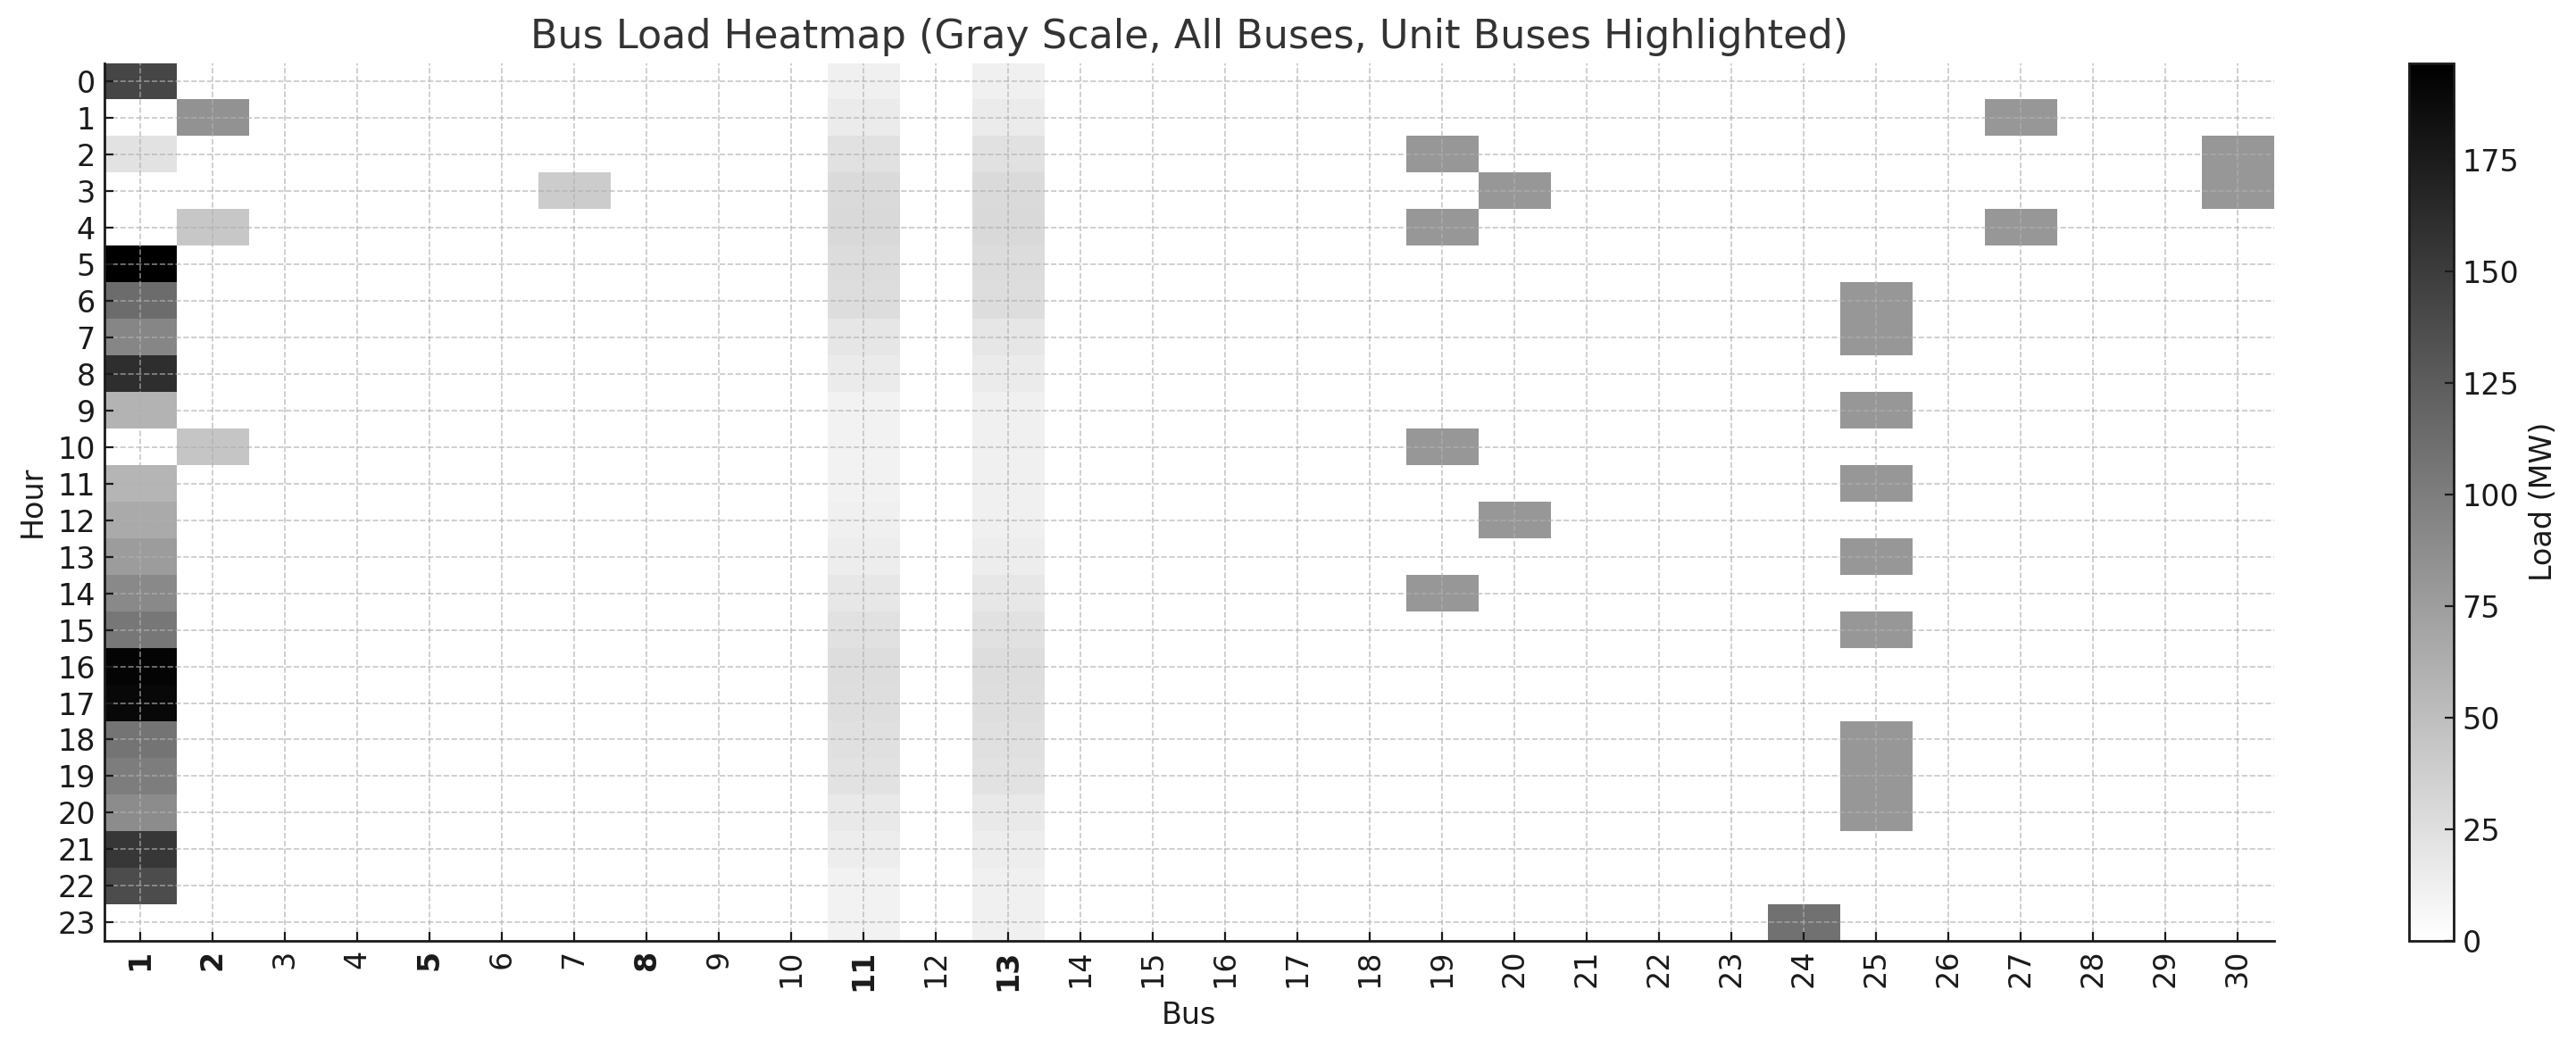
\includegraphics[width=0.85\textwidth]{figures/Q2-bus-load.png}
    \caption{Bus-level load allocation heatmap for Problem~2.}
    \label{fig:q2_bus}
\end{figure}
\noindent Figure~\ref{fig:q2_bus} uses 24 hours on the vertical axis and 30 buses on the horizontal axis, with darker shades indicating higher instantaneous demand; buses 1/2/24/25 turn dark during the morning and evening peaks and fade at midday and night. This spatial concentration shows that flexible load clusters around a few hubs, signaling the need to place reserve and flow buffers near these nodes in Problem~2 so that local voltage angles do not jump when an N--1 cut occurs.

\begin{figure}[htbp]
    \centering
    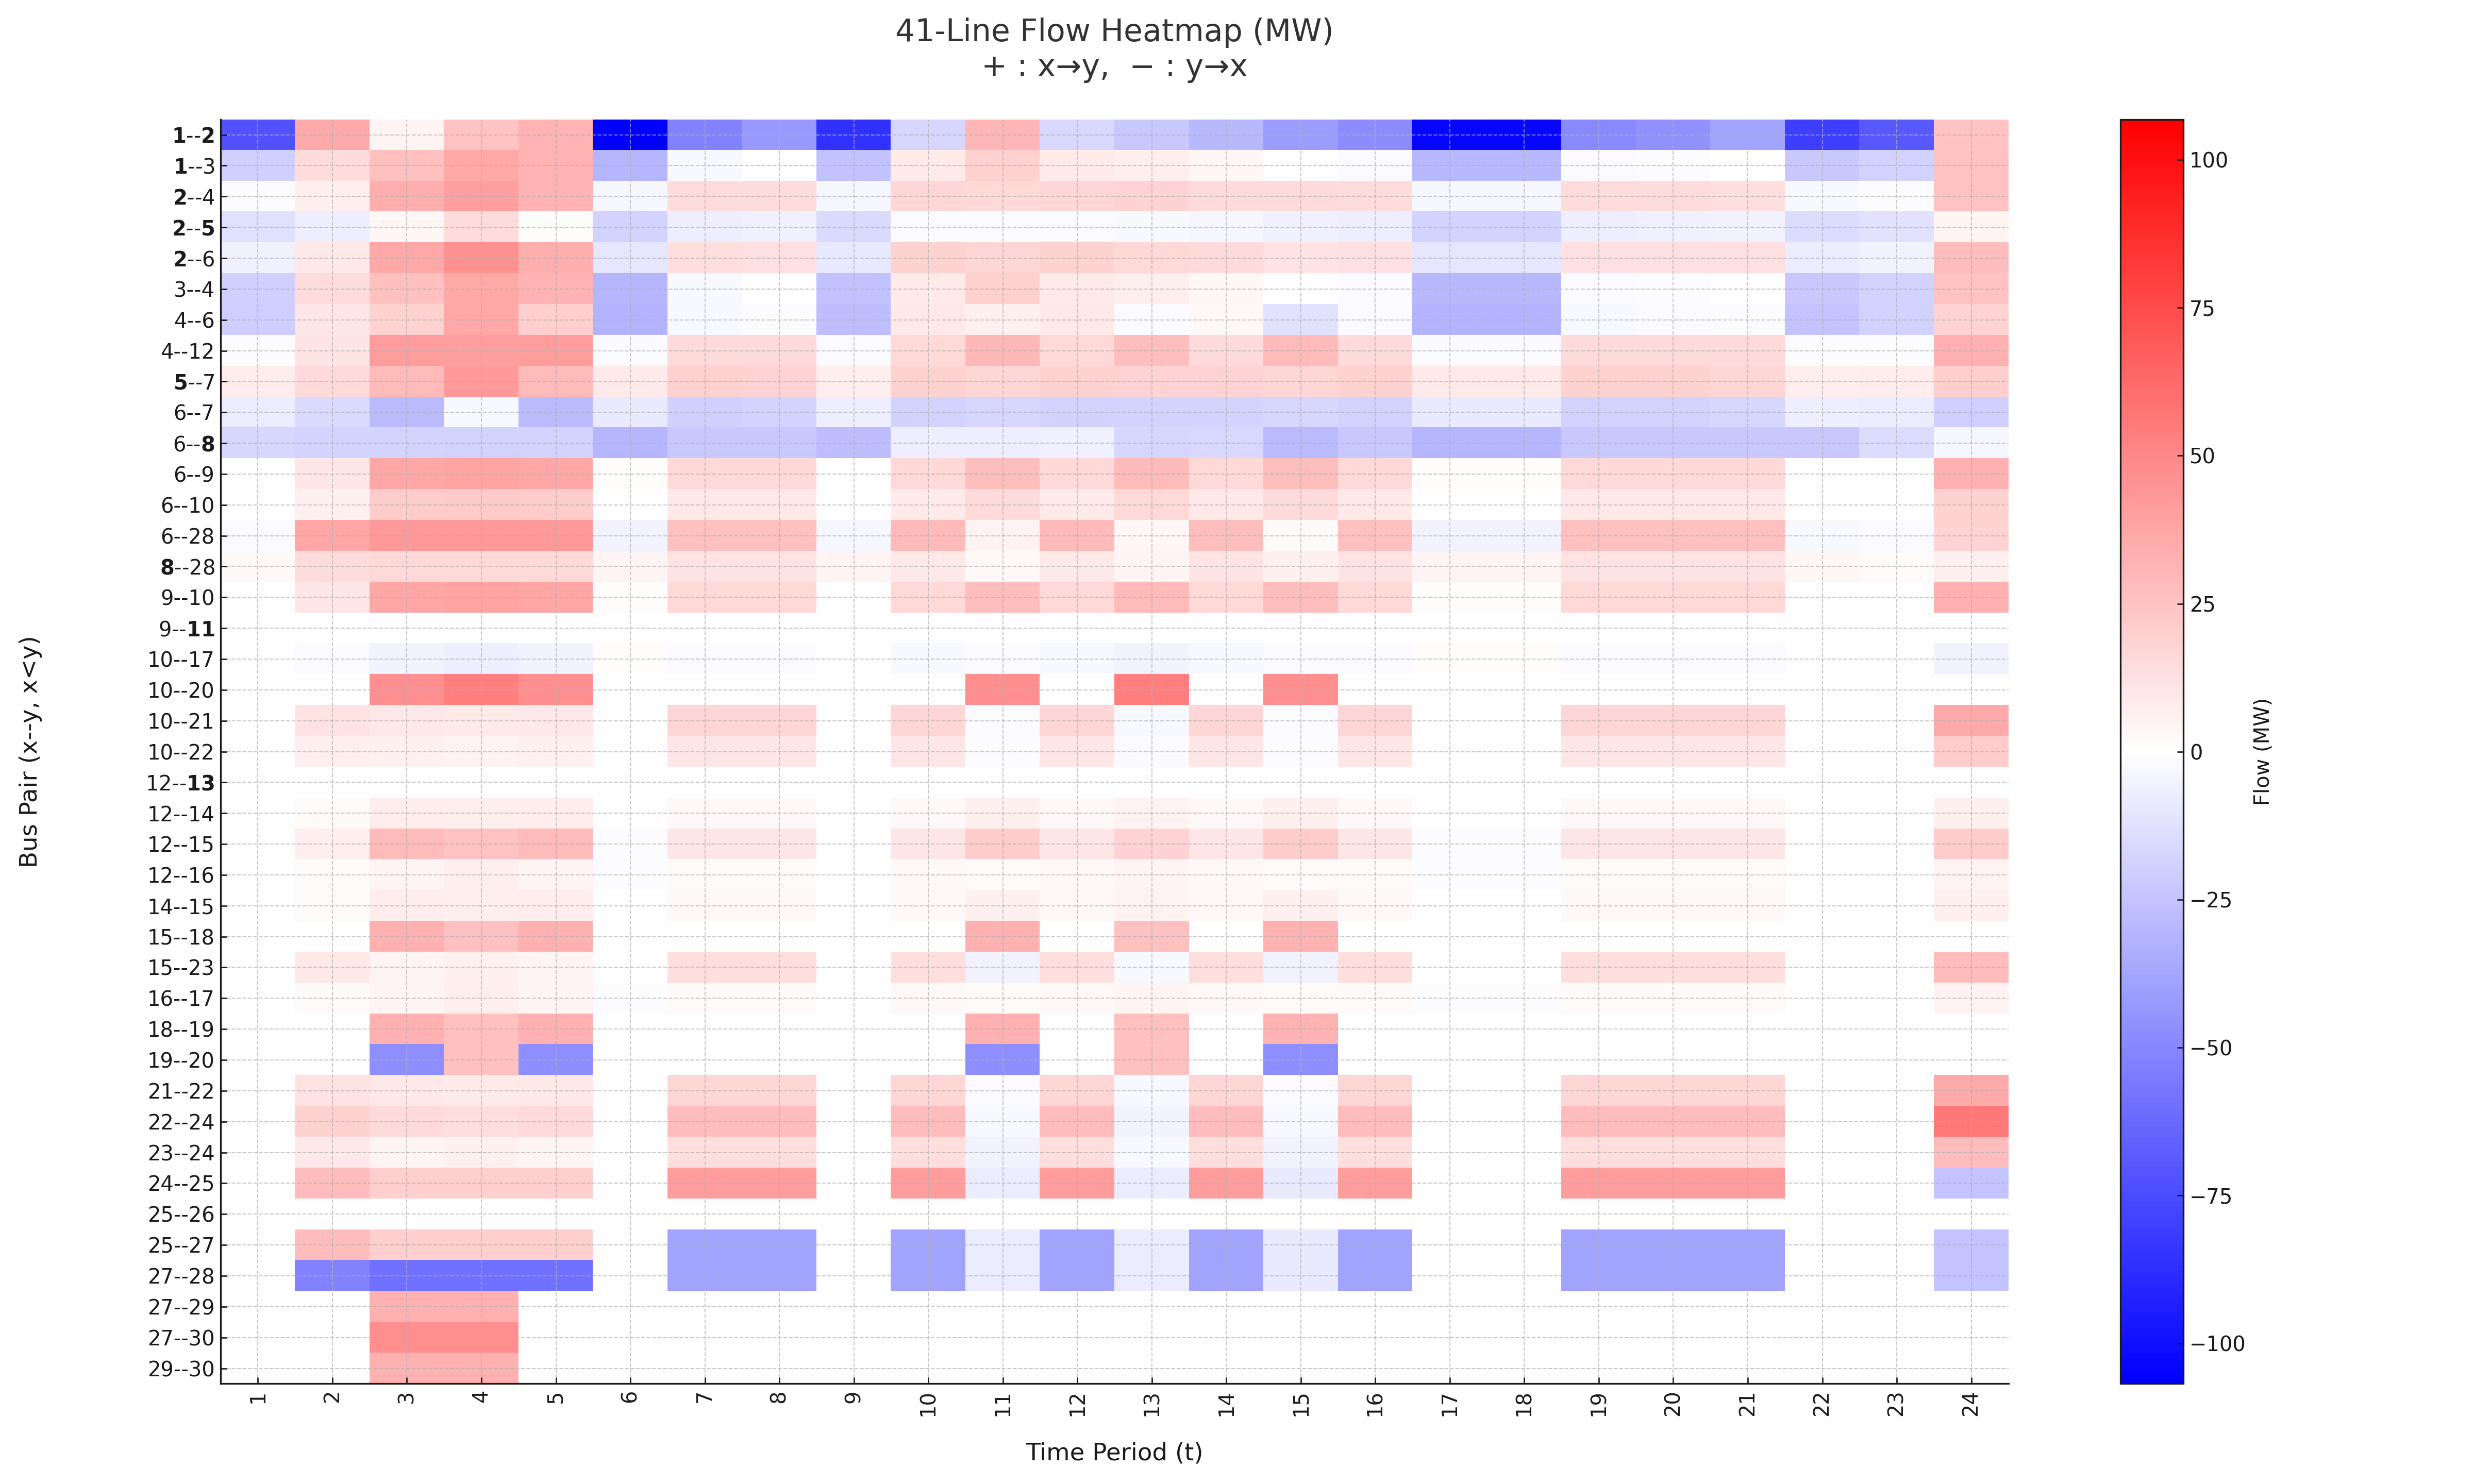
\includegraphics[width=0.85\textwidth]{figures/Q2-flow.png}
    \caption{Line-flow heatmap indicating direction reversals on main corridors.}
    \label{fig:q2_flow}
\end{figure}
\noindent Figure~\ref{fig:q2_flow} plots time on the horizontal axis and 41 transmission lines on the vertical axis, using a red/blue scale to show flow direction and magnitude; main corridors 1--2, 2--5, and 5--7 flip colors during hours 5--8 and 17--20, indicating bidirectional reversals at peaks. This behavior demonstrates that once network constraints enter, dispatch is no longer purely cost-driven but must preload critical corridors with margin so that Problem~2 satisfies the flow limits.

\begin{figure}[htbp]
    \centering
    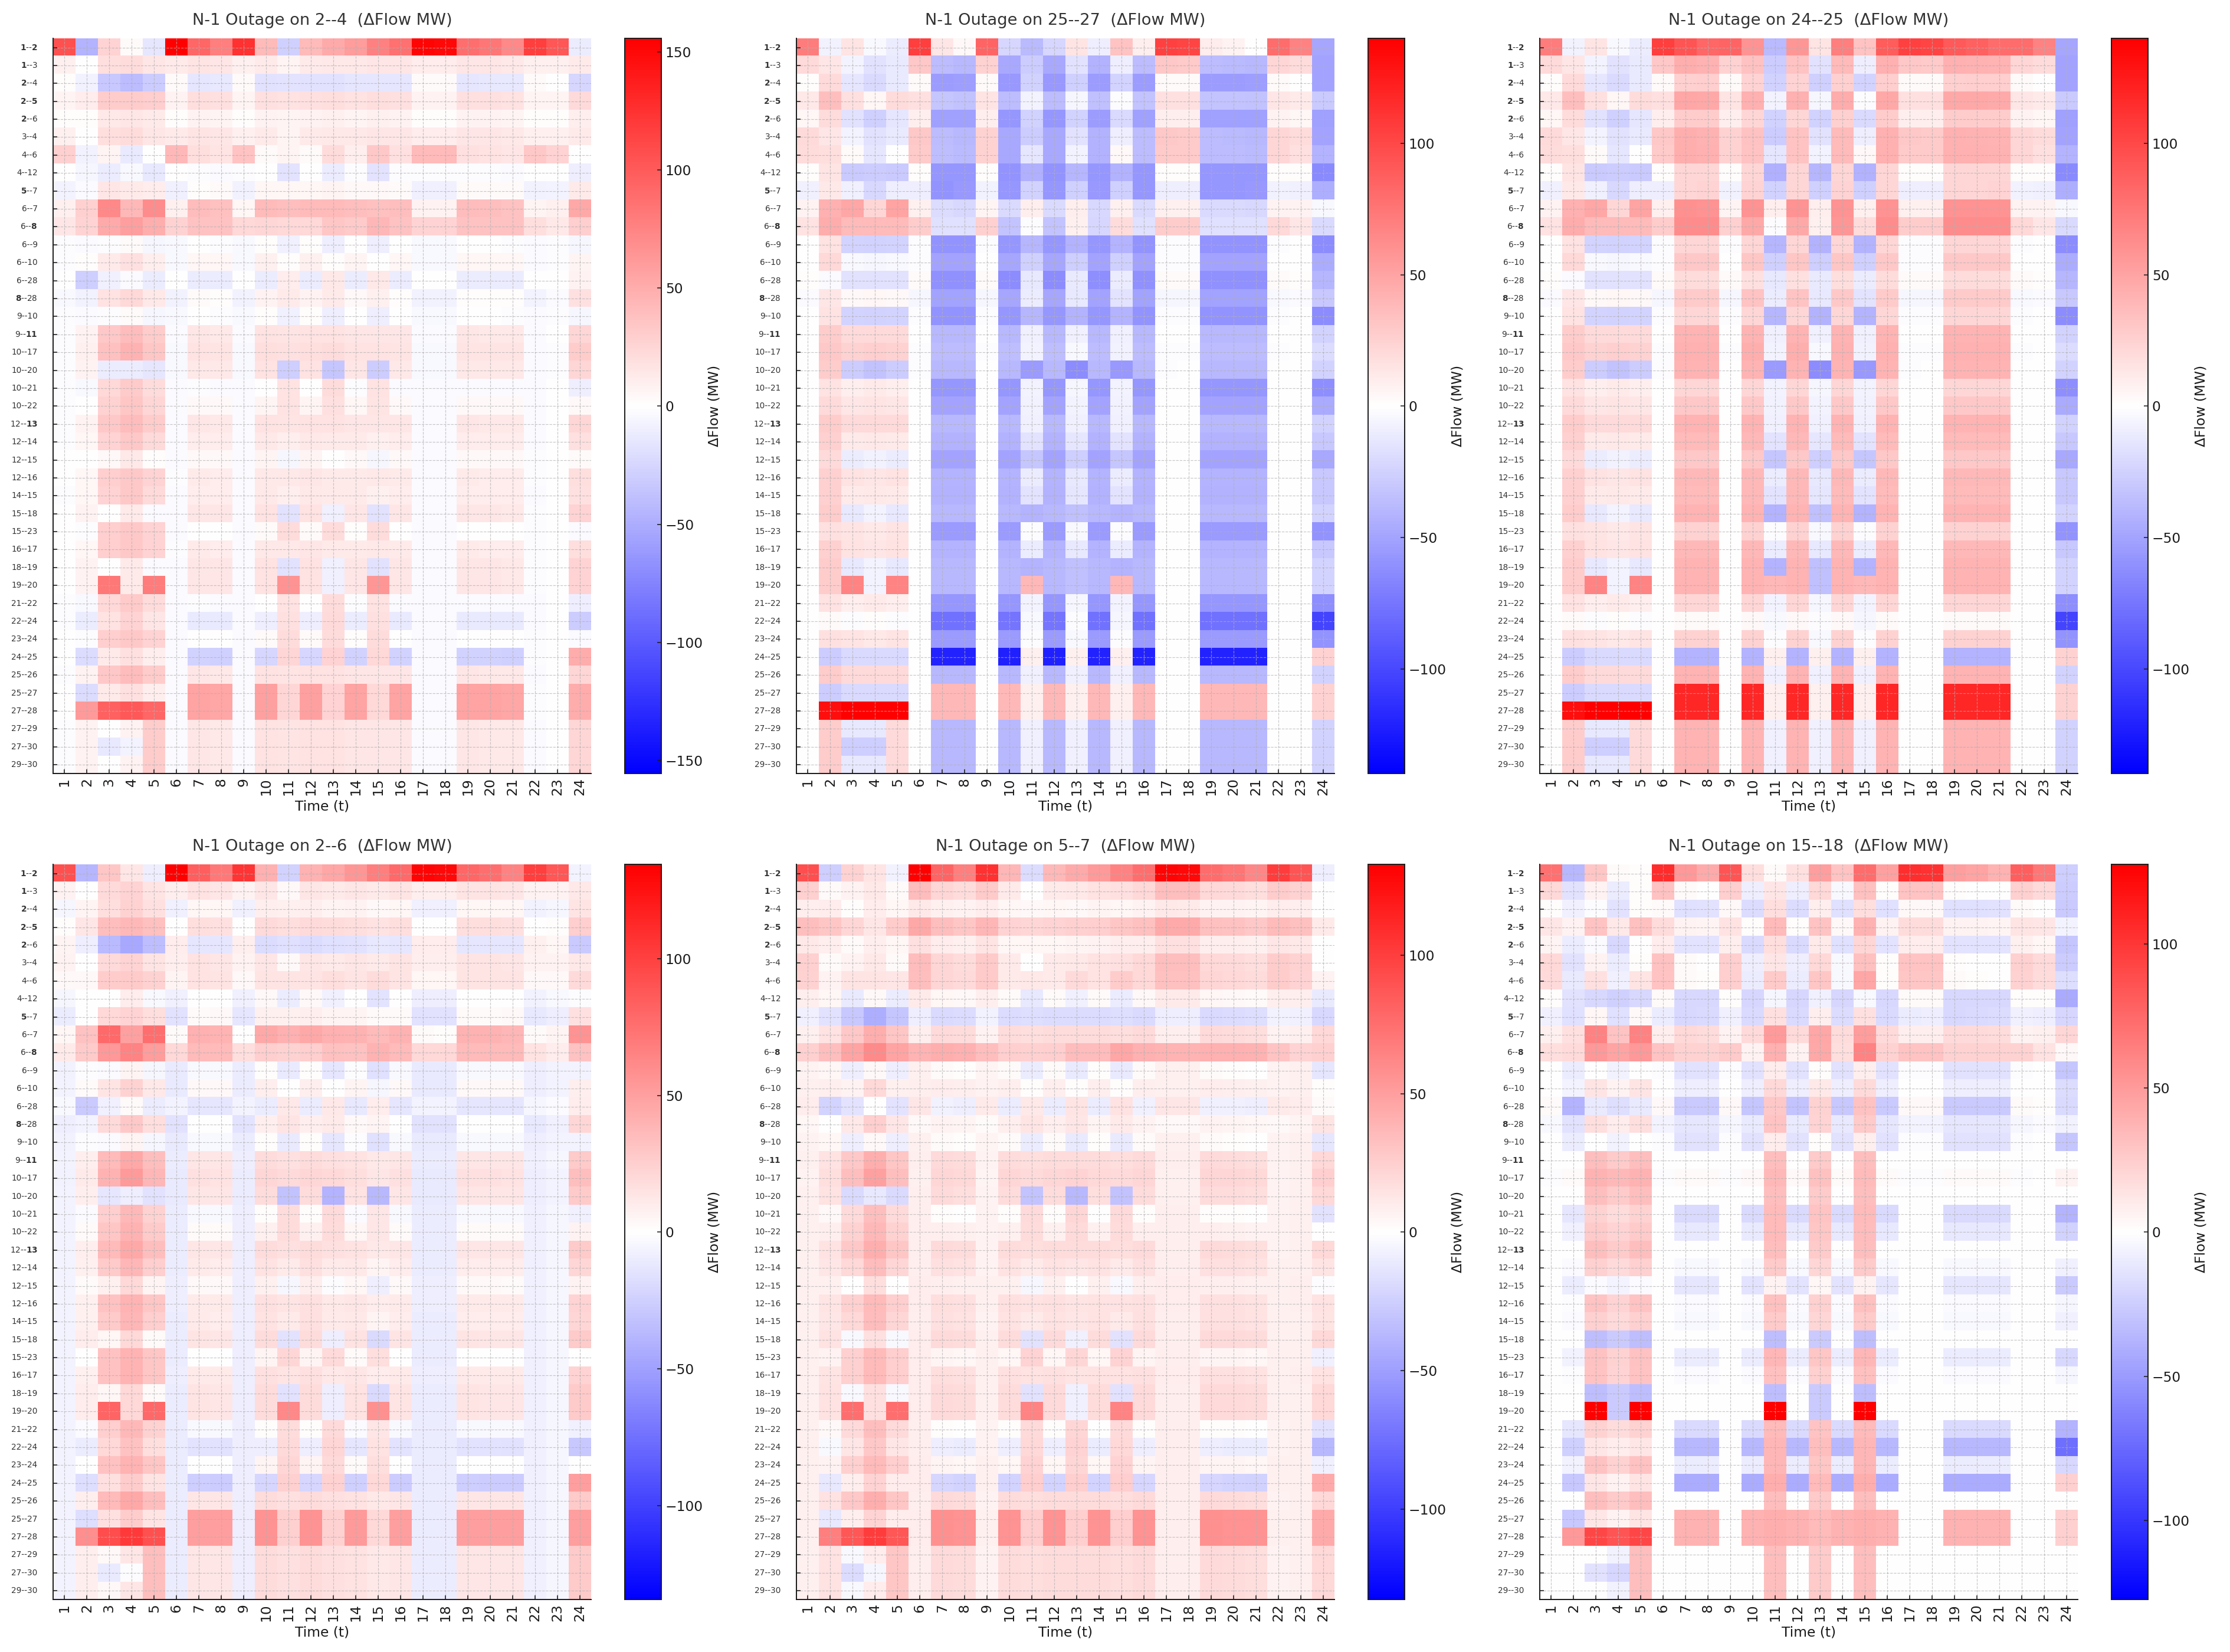
\includegraphics[width=0.85\textwidth]{figures/Q2-flow-outage-flow.png}
    \caption{$\Delta$flow patterns under N--1 line outages; deep colors show substitute corridors.}
    \label{fig:q2_flow_outage}
\end{figure}
\noindent Figure~\ref{fig:q2_flow_outage} plots a heatmap of flow deltas for every line contingency, with the color scale showing how each branch gains or sheds loading after the outage. Removing heavily loaded lines such as 2--6 or 24--25 turns nearby substitutes red while distant loops turn blue as they unload. This "geographic surrogate" pattern explains why security constraints keep adding cuts and serves as evidence for the need to diversify reserve geographically.

\begin{figure}[htbp]
    \centering
    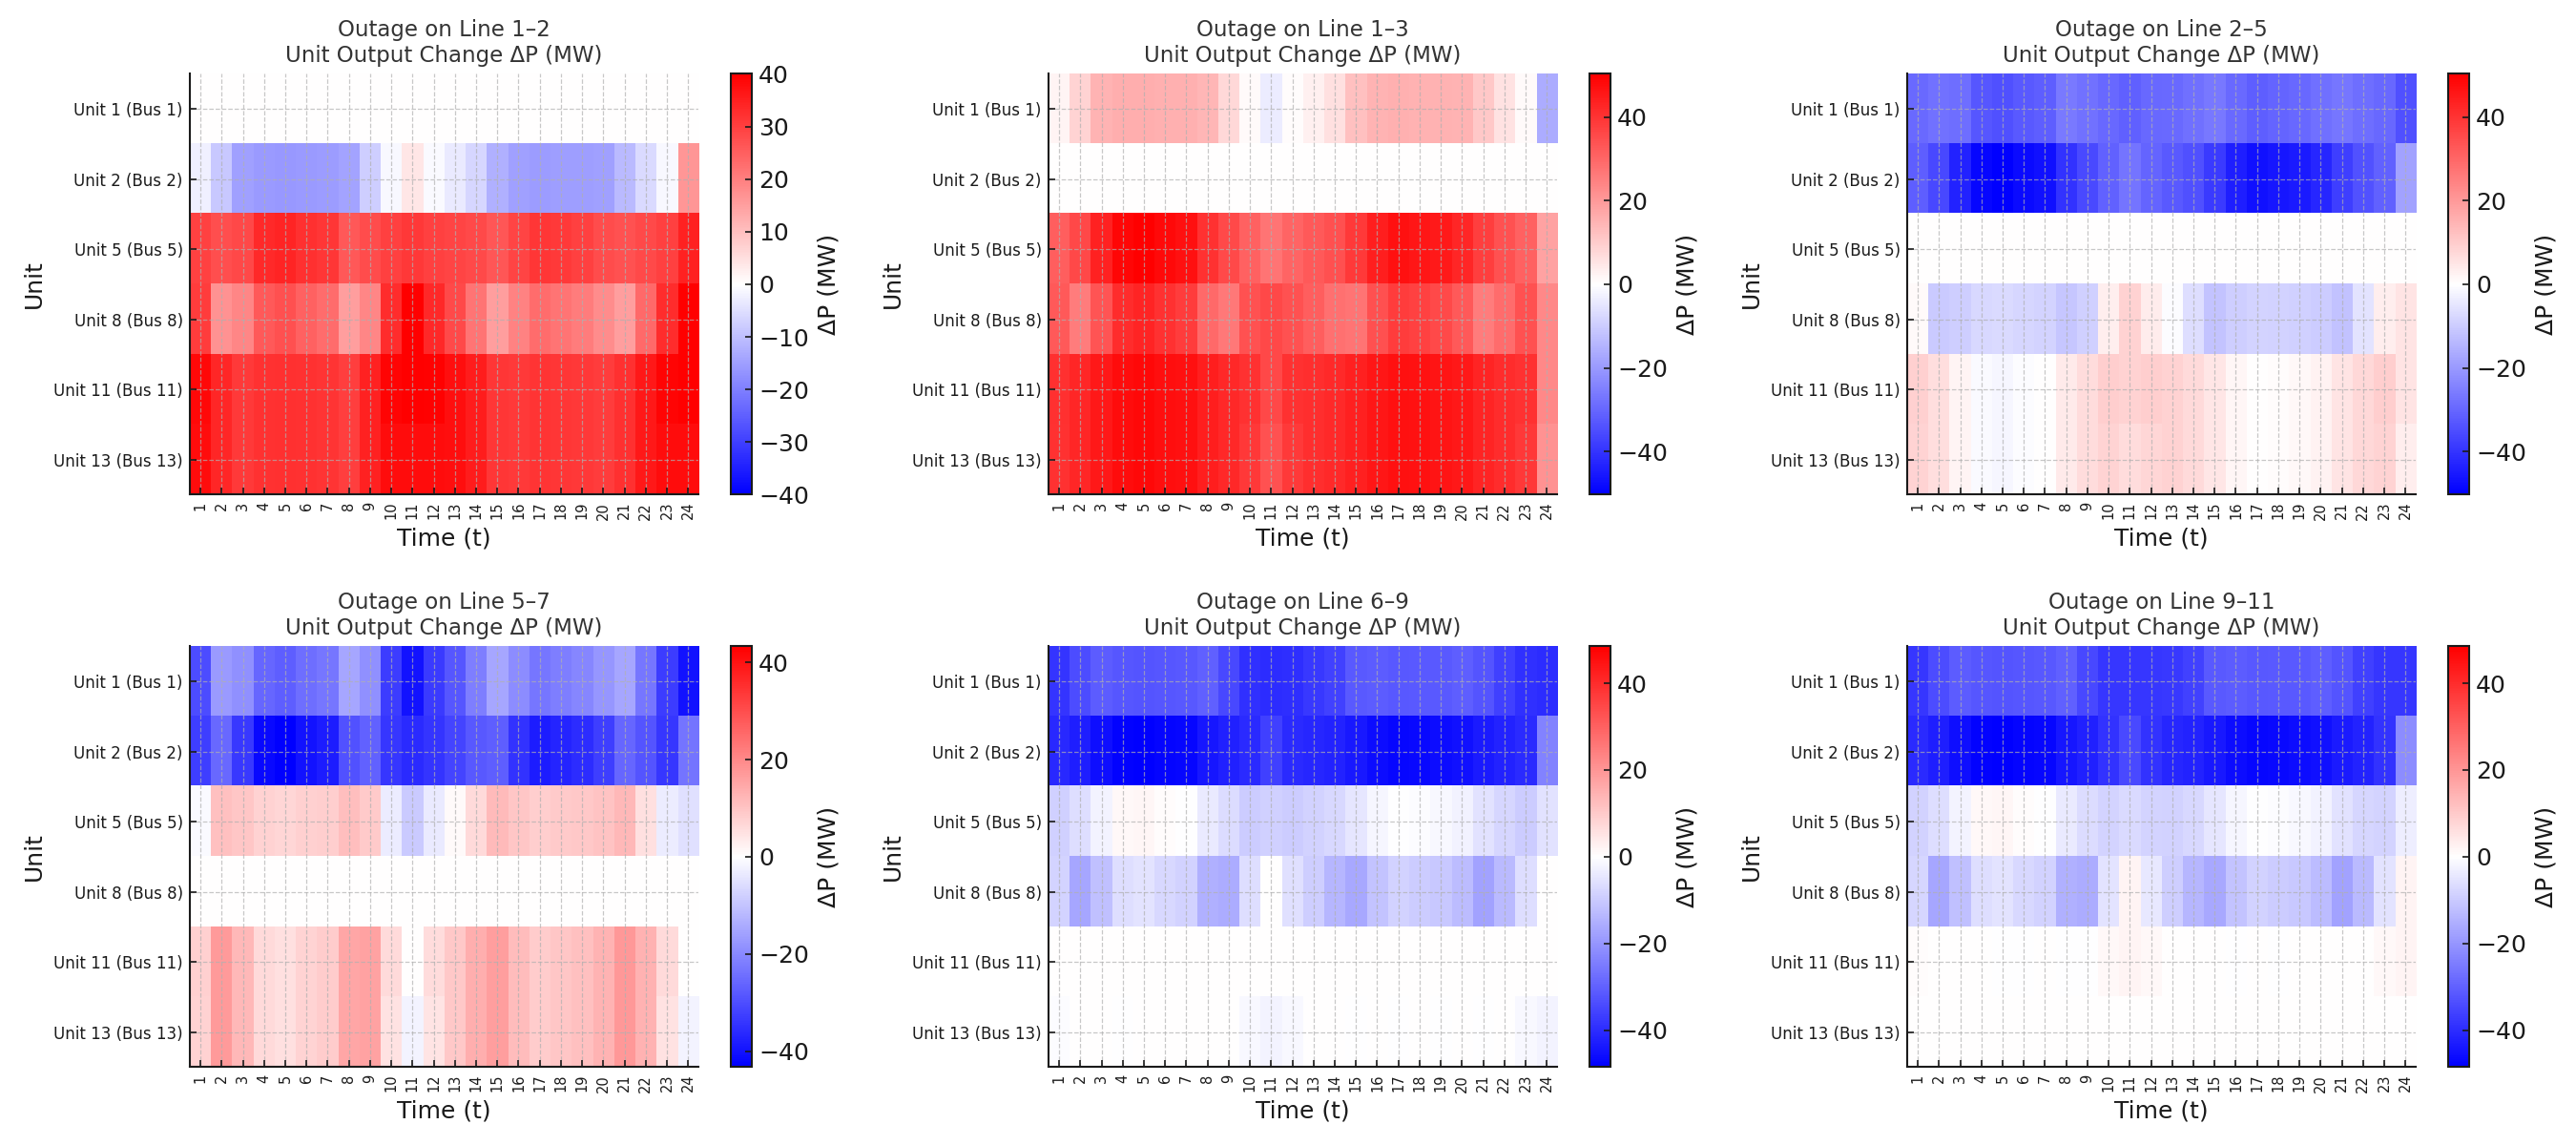
\includegraphics[width=0.85\textwidth]{figures/Q2-flow-outage-gen.png}
    \caption{Generator redispatch required after each line outage, emphasizing the burden on U1 and U2.}
    \label{fig:q2_flow_outage_gen}
\end{figure}
\noindent Figure~\ref{fig:q2_flow_outage_gen} uses line contingencies on the horizontal axis and generators on the vertical axis, with color showing each unit's compensating output $\Delta P$; U1/U2 appear dark red in almost every outage, whereas mid-system units respond strongly only when adjacent lines fail. This distribution indicates that the reserve constraint loads most of the compensation burden onto the largest units, motivating geographically diversified reserves in Problem~2 to reduce single-point risk.

\begin{figure}[htbp]
    \centering
    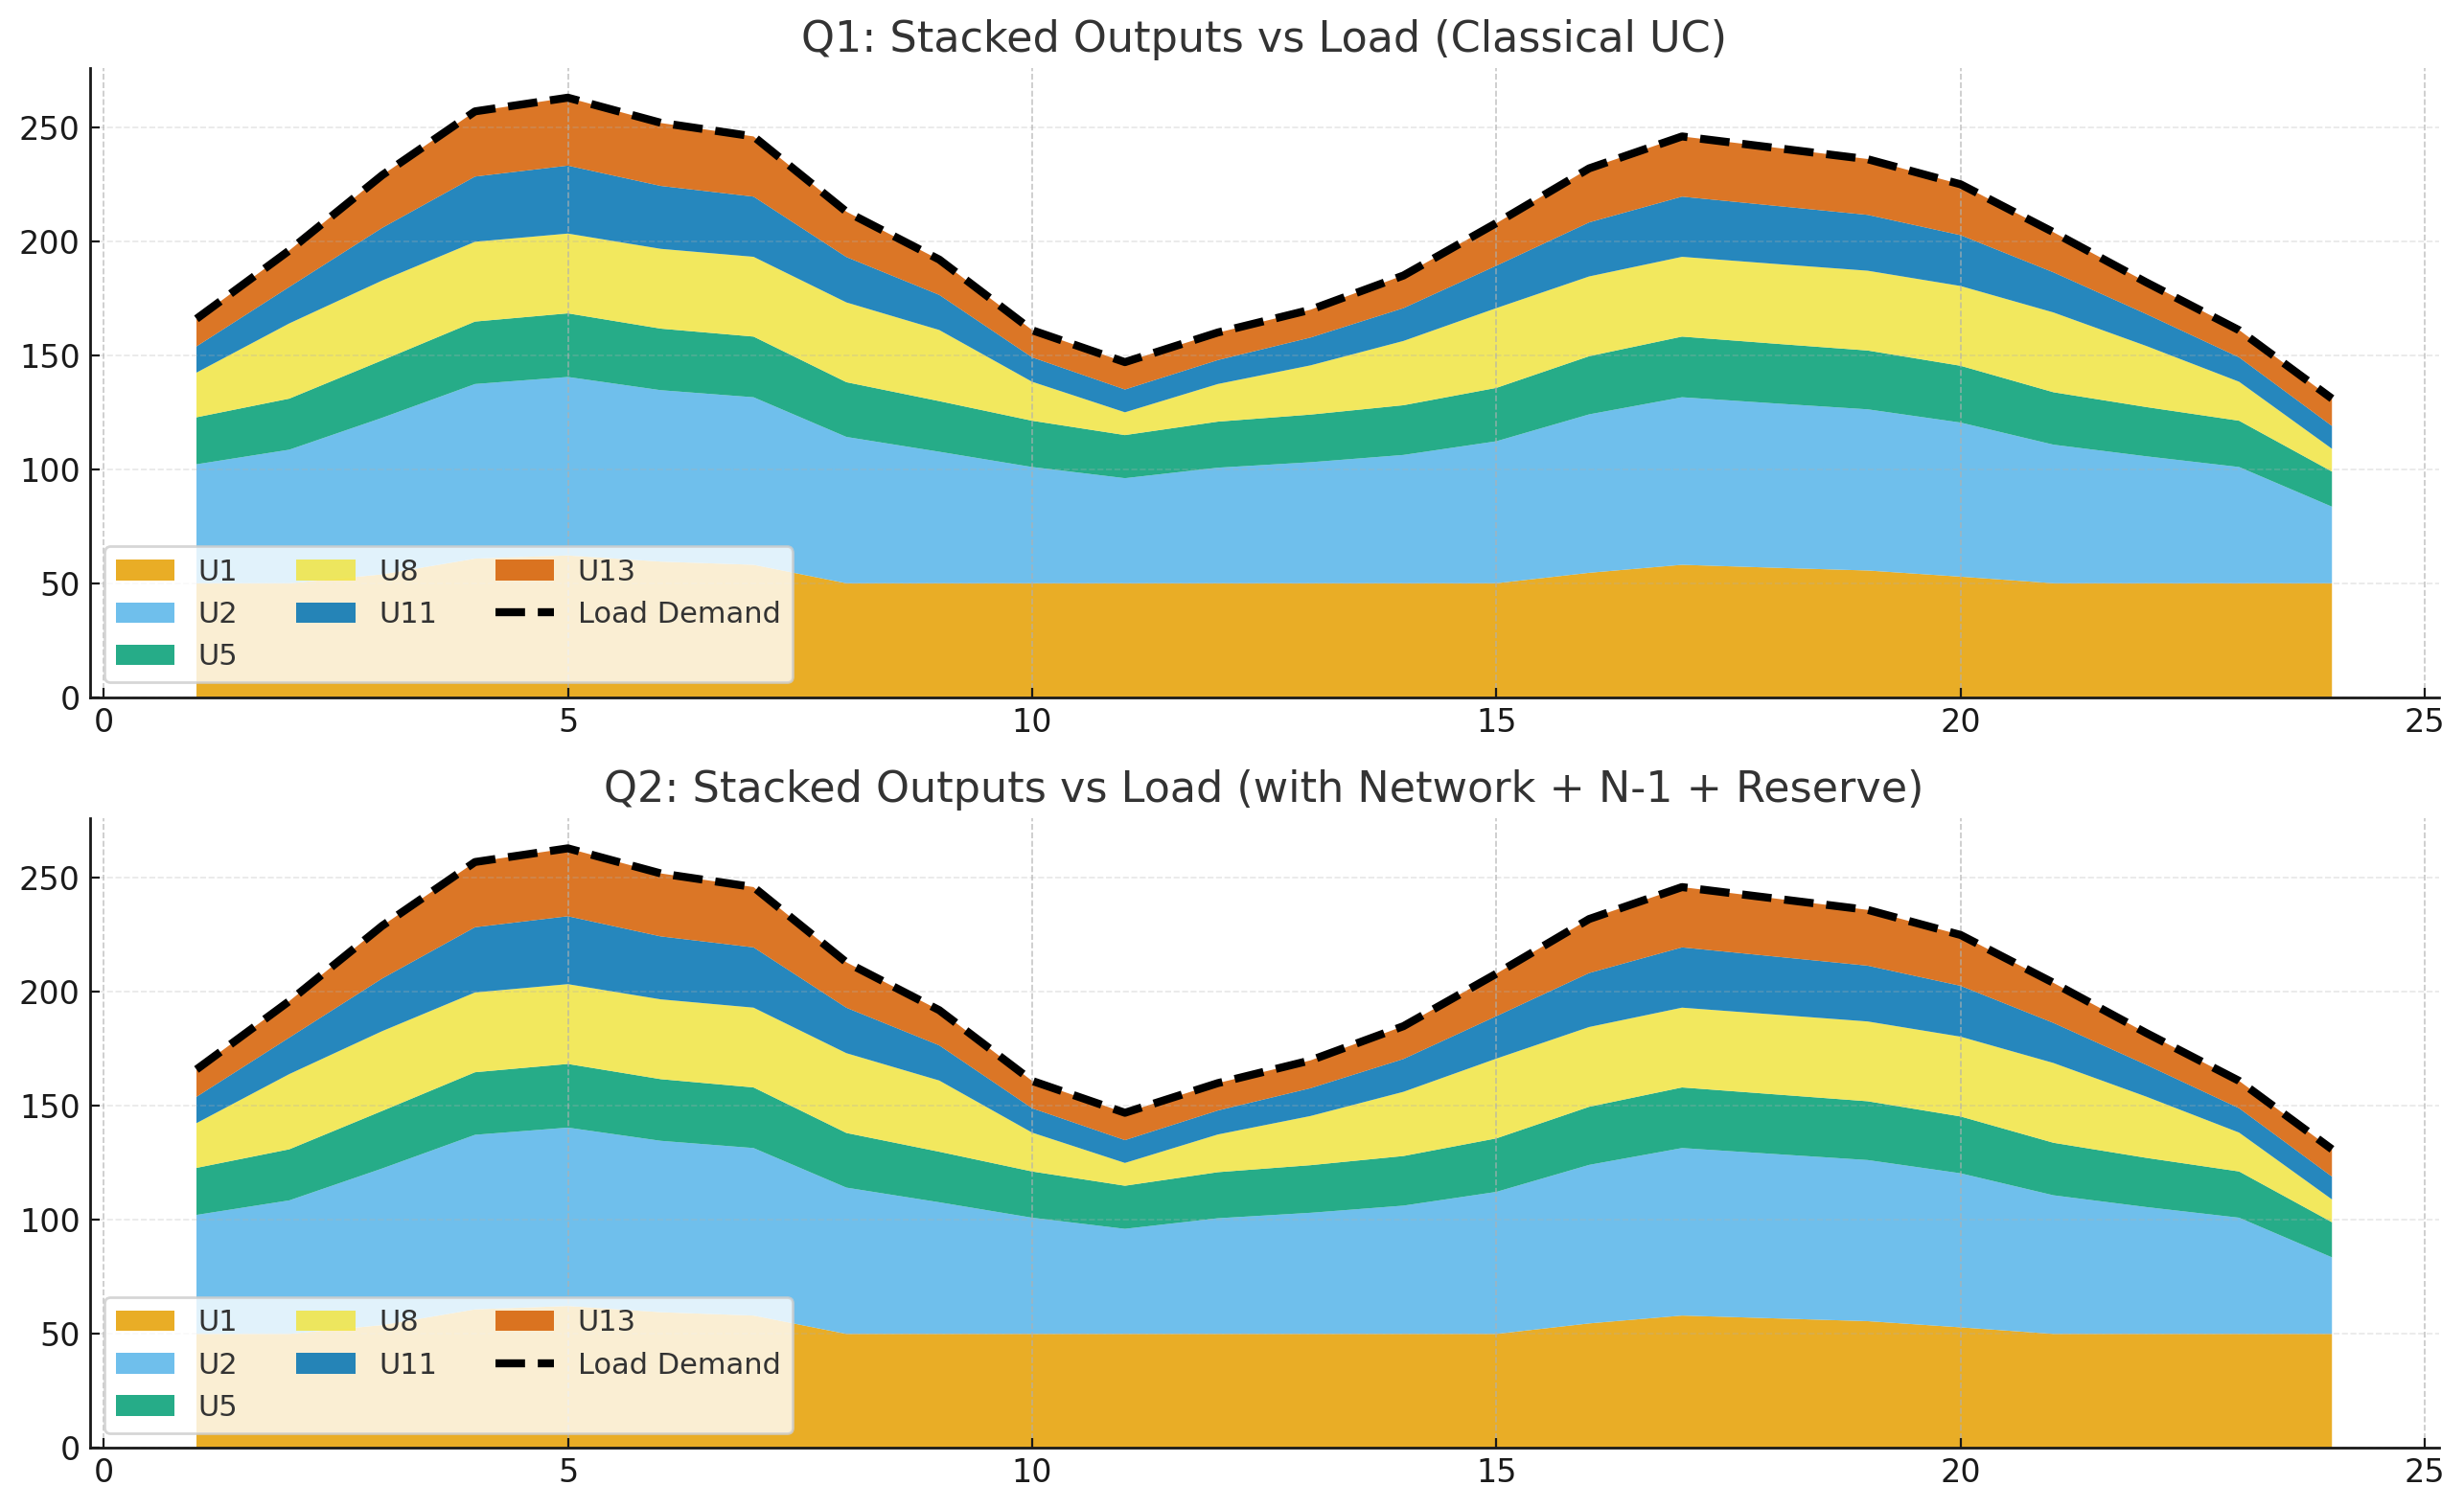
\includegraphics[width=0.75\textwidth]{figures/Q2-load.png}
    \caption{Stacked outputs comparison: Q1 (top) vs. Q2 (bottom) showing non-smooth dispatch once network limits apply.}
    \label{fig:q2_load}
\end{figure}
\noindent Figure~\ref{fig:q2_load} presents stacked curves with time on the horizontal axis, colored bands for unit power, and a dashed line for total load; the upper panel (Q1) remains smooth, whereas the lower panel (Q2) shows jagged additions around hours 6, 14, and 19. This comparison demonstrates that network and N--1 constraints force some units to hold higher output during low-load periods to maintain flow feasibility and reserve margins.

\begin{figure}[htbp]
    \centering
    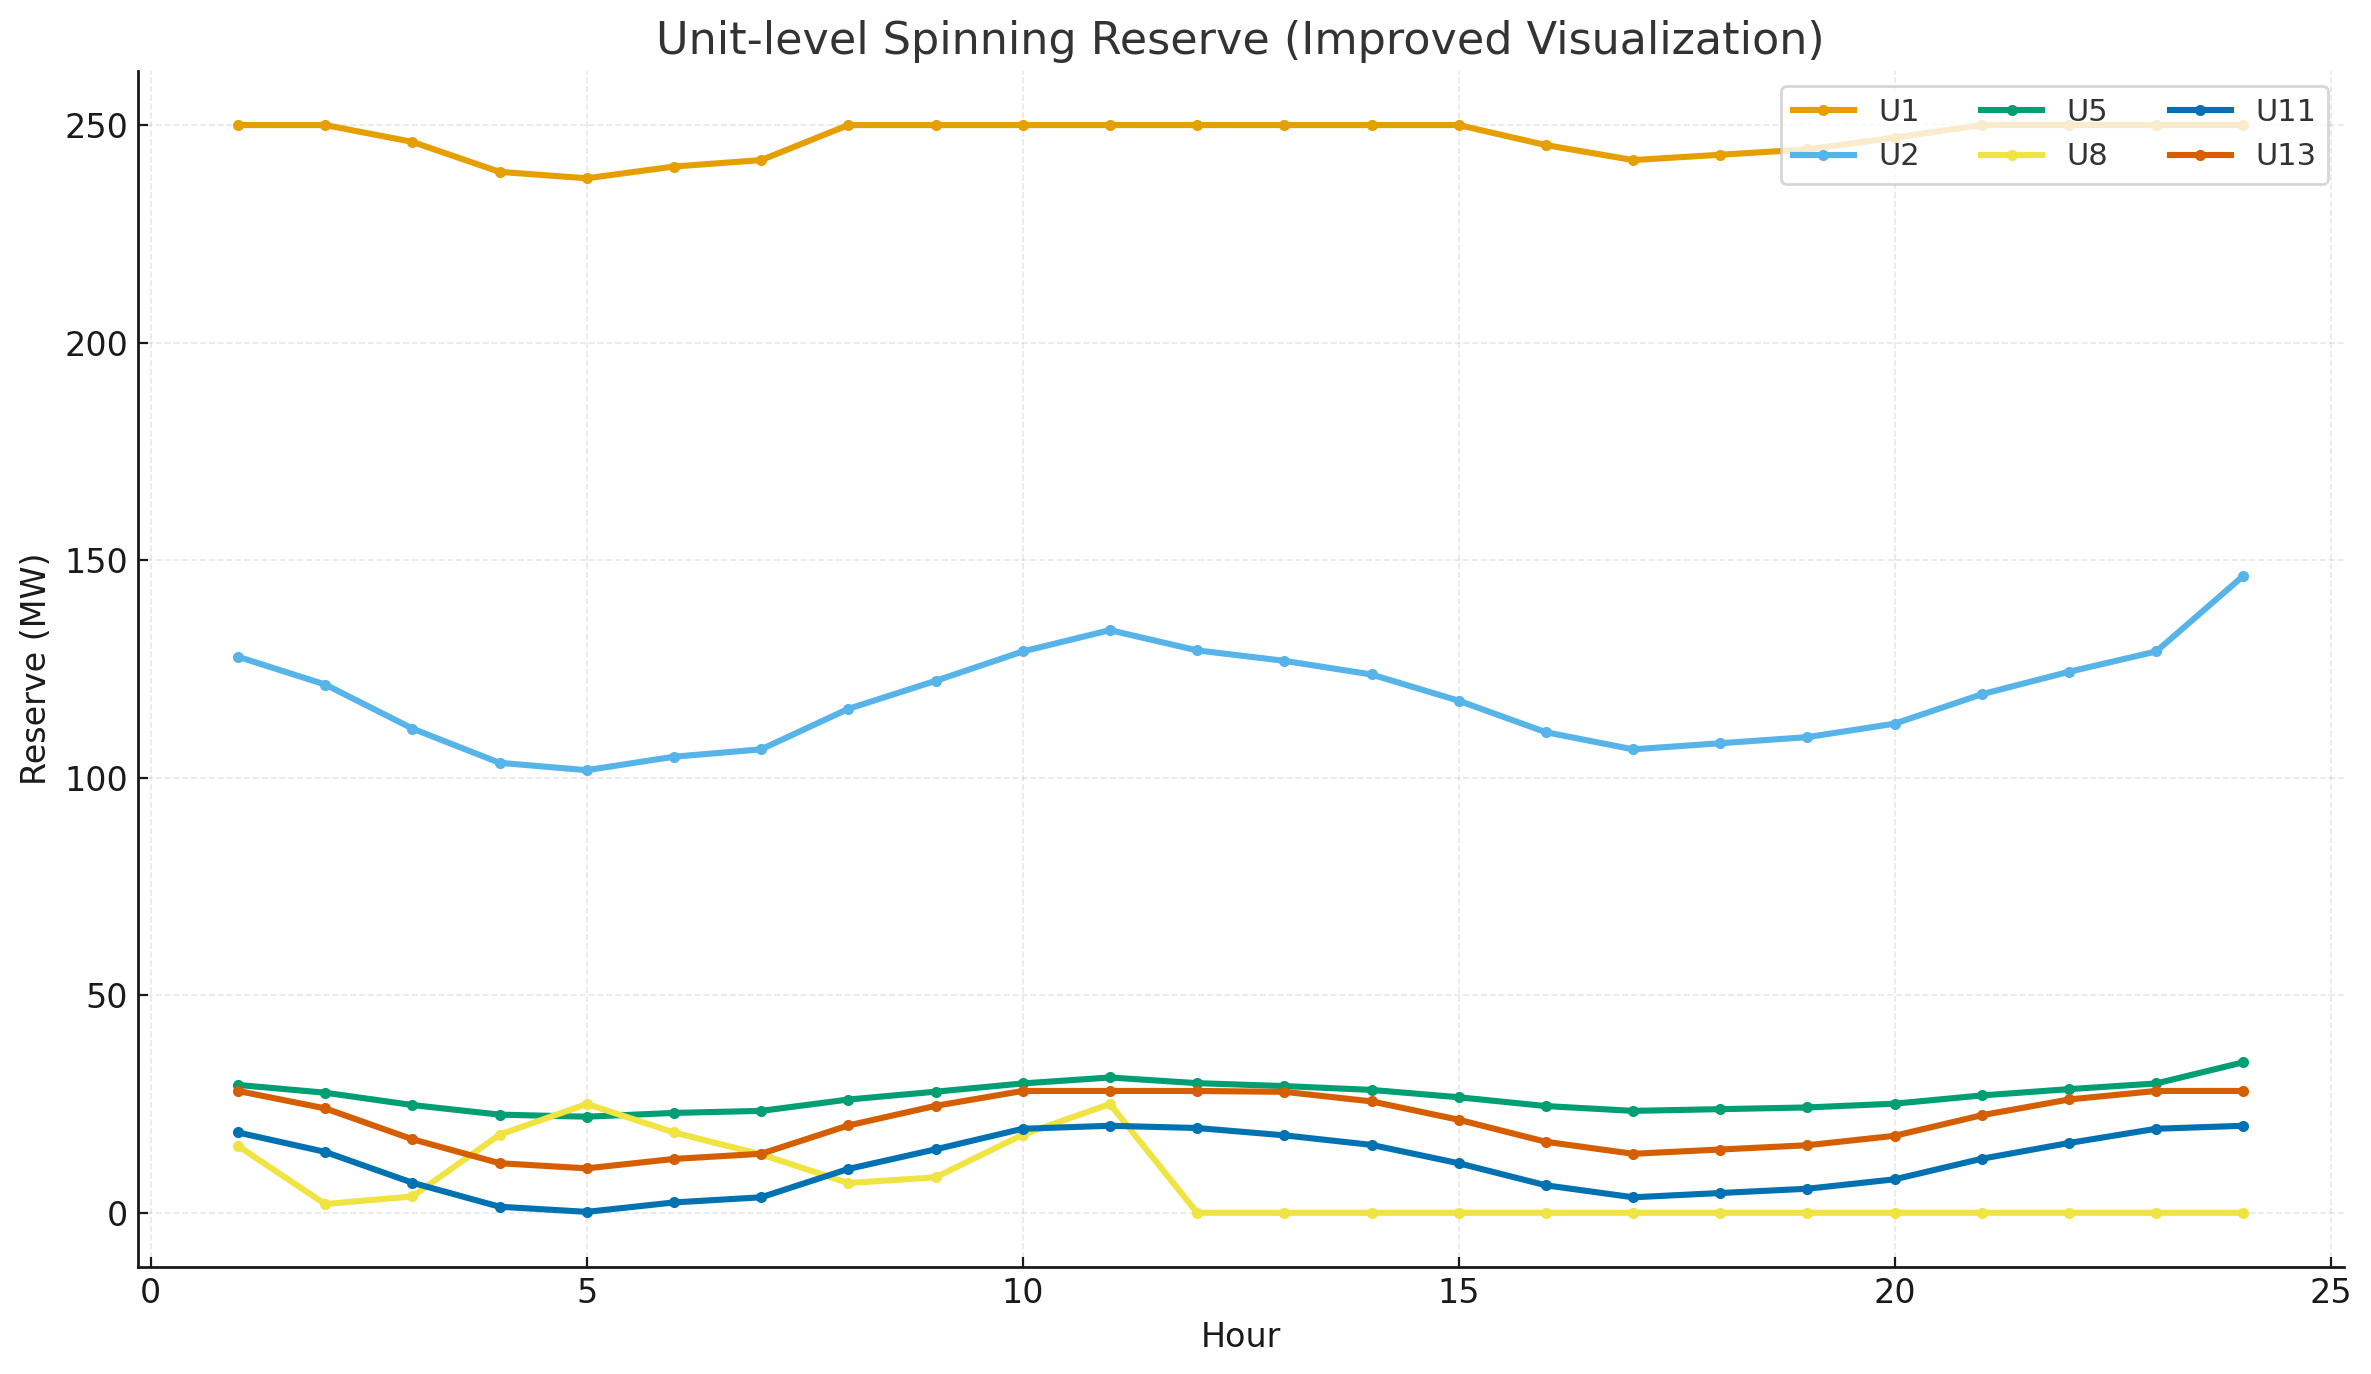
\includegraphics[width=0.7\textwidth]{figures/Q2-reserve.png}
    \caption{Unit-level spinning reserve showing that U1 and U2 naturally hold most of the contingency headroom.}
    \label{fig:q2_reserve}
\end{figure}
\noindent Figure~\ref{fig:q2_reserve} uses time on the horizontal axis and colored bars for each unit, with the vertical value equal to spinning reserve; U1 supplies roughly 240--250~MW, U2 about 100--140~MW, and the remaining units mostly stay below 30~MW while following the load's twin peaks. Even without a fixed system-wide quota, the plot shows that the baseload units shoulder nearly all available headroom, so the N--1 strategy in Problem~2 must prioritize preserving their margin when adding contingency cuts.

\section{Problem 3: QUBO Transformation and Quantum Solution}

\subsection{Binary encoding and penalties}
Continuous variables are discretized via binary expansions such as
\begin{equation}
    \label{eq:q3_encoding}
    P_{i,t} = P_i^{\min} u_{i,t} + \sum_{k=0}^{K_P-1} \delta_{P,k} x^{(P)}_{i,t,k}, \quad x^{(P)}_{i,t,k}\in\{0,1\}.
\end{equation}
\noindent Equation~\eqref{eq:q3_encoding} states that each analog dispatch level is reconstructed by anchoring at the committed minimum $P_i^{\min} u_{i,t}$ and then adding weighted binary digits $\delta_{P,k}$ chosen by $x^{(P)}_{i,t,k}$, so every MW ladder rung maps to a specific subset of bits, following the standard Ising reformulation template in~\cite{lucas2014}.
The same encoding applies to ramp, balance, and other slack variables so that every inequality maps a bit flip to a physical jump on the Kaiwu CIM Ising nodes, matching the discrete transitions observed in the Q3 quantum traces.
Slack variables for inequalities follow the same pattern so that every constraint can be squared and added to the energy matrix. The complete QUBO is
\begin{equation}
    \label{eq:q3_qubo}
    Q = Q_{\text{cost}} + \lambda_{\text{bal}} Q_{\text{bal}} + \lambda_{\text{lim}} Q_{\text{lim}} + \lambda_{\text{log}} Q_{\text{log}} + \lambda_{UT} Q_{UT} + \lambda_{DT} Q_{DT} + \lambda_{\text{ramp}} Q_{\text{ramp}}.
\end{equation}
\noindent Equation~\eqref{eq:q3_qubo} assembles the energy matrix by stacking the quadratic objective block $Q_{\text{cost}}$ with penalty blocks for balance, limits, logic, minimum up/down, and ramp violations, each modulated by its weight $\lambda_{\bullet}$.
Following the internal Problem~3 notes and the Q3 comparison plots, we tune penalties in an ascending sequence (balance -> limit -> logic -> time constraints -> ramp) so that the residuals (41.81~MW, 70.99~MW, 82.22~MW) strike a workable compromise with quantum hardware noise.
Because all components share the same binary vector from Equation~\eqref{eq:q3_encoding}, increasing any $\lambda_{\bullet}$ tightens the corresponding feasible basin but pushes the 7,024-bit matrix closer to the Kaiwu density ceiling, motivating the reduction workflow in Problem~4.

\subsubsection*{Model Core}
Slack variables $s_{\text{bal},t}, s_{\text{ramp},i,t}, s_{UT,i,t}$ are introduced by first writing each inequality in its UC form (e.g., $\sum_i P_{i,t}-D_t + s_{\text{bal},t}=0$) and then discretizing $s$ with the same binary ladder as Equation~\eqref{eq:q3_encoding}. Physically, $s_{\text{bal},t}$ records power deficits or surpluses and corresponds to the balance slack in the classical UC, while $s_{\text{ramp},i,t}$ measures the buffering stroke when a unit exceeds $RU_i$ or $RD_i$. Embedding these slack registers alongside $u_{i,t}$ and $P_{i,t}$ gives every UC constraint an "absorption" path so that quantum states perturbed by mild noise are not discarded outright.
The 7{,}024-bit Hamiltonian is organized in contiguous blocks: the first $24\times |\mathcal{I}|$ bits store classical ON/OFF states $u_{i,t}$, the next $24\times |\mathcal{I}|\times K_P$ bits encode dispatch magnitudes $P_{i,t}$, and the remaining roughly 30\% bits house the multi-family slack registers. Compared with the classical UC basis where $u_{i,t}$ and $P_{i,t}$ are hybrid binary/continuous, this ``u-P-slack'' segmentation explicitly dedicates bit budget to constraint buffers, which is rarely detailed in the existing UC-to-QUBO literature.
Constraint absorption relies on a hierarchical penalty stack: $\lambda_{\text{bal}}$ is tuned first (set to $8\times$ the fuel quadratic curvature) to force near-feasible power balance, then $\lambda_{\text{lim}}$ and $\lambda_{\text{log}}$ are escalated to suppress physical limit and logic errors, while $\lambda_{UT}, \lambda_{DT}$, and $\lambda_{\text{ramp}}$ are gradually increased until slack occupancy shrinks below 10\% in the annealing samples. This staged tuning ensures that penalties do not overwhelm the objective yet remain strong enough to ``absorb'' power balance, ramp, and minimum-time violations, echoing the QUBO modeling guidelines summarized in~\cite{glover2018} and contrasting with Problem~1 where feasibility is guaranteed by the MIP solver rather than by energy shaping.
Despite the slack cushions, the Problem~3 log reports residuals of 41.81~MW (balance) and 82.22~MW (ramp). These arise when annealed states prefer to flip slack bits instead of coordinating $u$/$P$ blocks, especially in hours with steep load ramps. Consequently we use the recorded $s_{\text{bal},t}$ values during classical post-processing, feed the high-residual periods back into the Gurobi model, and resolve to restore the zero-residual baseline from Problem~1. This mechanism highlights how the slack/penalty combination both enables quantum feasibility and necessitates classical correction, marking a divergence from prior art that assumes penalty terms alone can drive residuals to zero.

\subsection{Kaiwu workflow}
The pipeline builds $Q$, attempts to submit it to the Kaiwu CIM hardware, falls back to simulated annealing when the queue rejects the job, decodes the returned Ising vector into UC variables, and re-evaluates constraint residuals. Detailed summaries are archived for analysis and comparison.

\subsection{Result comparison}
To highlight the differences between Problem~1 (classical UC) and Problem~3 (QUBO) in the behavior of $u_{i,t}$ and $P_{i,t}$, we aggregate the solver logs and exported variables to compute average outputs for representative peak hours (t=8--12) and valleys (t=20--23), along with start/stop counts, maximum ramps, balance residuals, and QUBO bitwidth data.

\begin{table}[htbp]
    \centering
    \caption{Problem~1 vs. Problem~3 aggregated $u_{i,t}/P_{i,t}$ metrics}
    \label{tab:q3_compare}
    \begin{tabular}{@{}>{\raggedright\arraybackslash}p{5.8cm}cc@{}}
        \toprule
        Metric & Classical UC (Problem~1) & QUBO (Problem~3) \\
        \midrule
        Average output at representative peak (t=8--12) (MW) & 174.6 & 204.4 \\
        Average output at representative valley (t=20--23) (MW) & 193.1 & 221.3 \\
        Total start/stop count & 0 & 72 \\
        Maximum ramp (MW) & 17.4 (U2, 23$\rightarrow$24) & 142.9 (U1, 19$\rightarrow$20) \\
        Power-balance residual $\max|\text{res}|$ (MW) & 0 & 41.81 (t=08) \\
        QUBO bitwidth / density & 432 bin + 144 cont vars & 7{,}024 bits / $6.65\times 10^{-4}$ \\
        \bottomrule
    \end{tabular}
\end{table}

\noindent Table~\ref{tab:q3_compare} shows that the quantum solution keeps more than 221~MW of average output during valleys, executes 72 start/stop events, and produces a 142.9~MW single-step ramp that flips $u_{i,t}$ states, yielding a 41.81~MW balance residual at $t=08$; the classical baseline, by contrast, satisfies zero residual and moderate ramps automatically via the MIP. The dashed trajectory in Figure~\ref{fig:q3_compare} matches these statistics, indicating that the reduced-bit QUBO still prefers bit flips over smooth dispatch, so Problem~3 must treat the quantum schedule as a heuristic seed and post-process it with the Problem~1 model to recover continuous feasibility.

\begin{figure}[htbp]
    \centering
    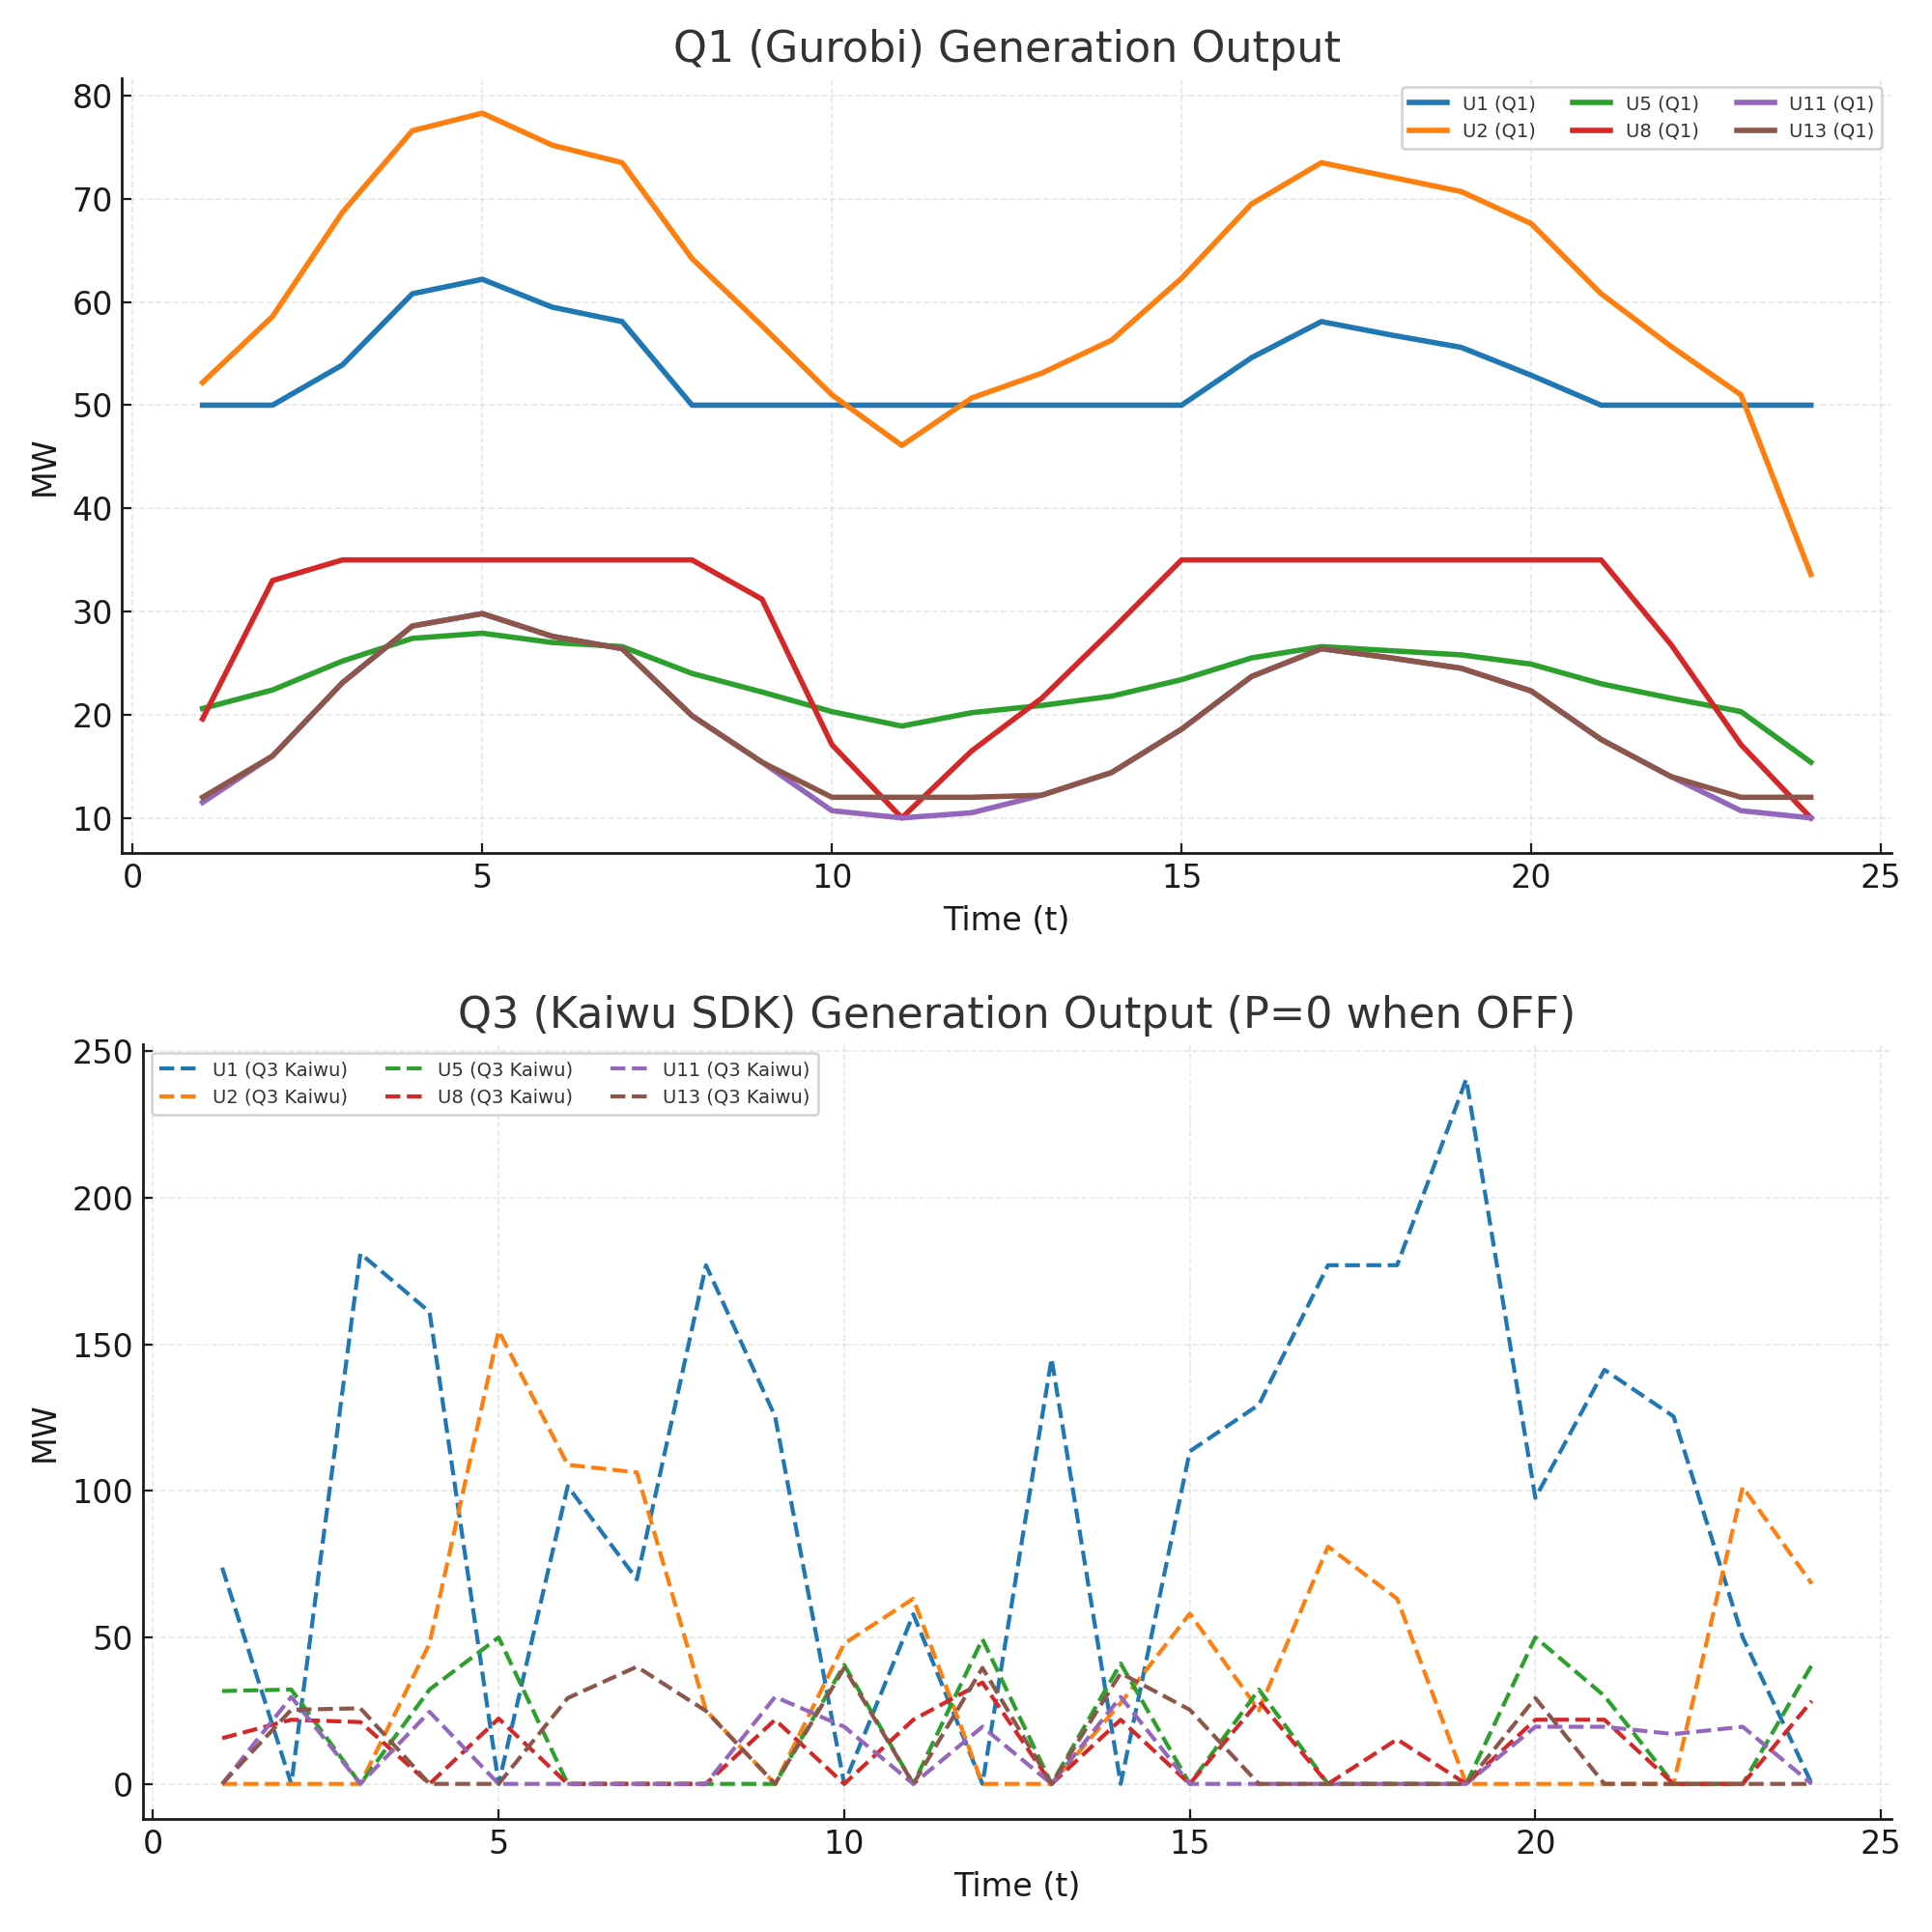
\includegraphics[width=0.85\textwidth]{figures/Q3.png}
    \caption{Comparison of classical (solid) and QUBO (dashed) dispatch illustrating the quantum solver's jumps.}
    \label{fig:q3_compare}
\end{figure}

\section{Problem 4: Scale Reduction and Feasibility}

\subsection{Reduction strategy}
Following the internal reduction memo\footnote{The internal reduction memo summarizes the heuristics for slack consolidation and bit-width pruning.} and the diagnostics from Problem~3, we:
\begin{enumerate}
    \item \textbf{Consolidate slack variables} so that each constraint family shares a limited set of penalty bits.
    \item \textbf{Trim bit-widths and time slices}, focusing on the peak hours that dominate feasibility and restricting power ranges to relevant bands.
    \item \textbf{Prune scenarios} by keeping only the most critical outages, thereby shrinking $Q$ to 435 bits that the Kaiwu hardware can host.
\end{enumerate}

\subsection{Results}
The reduced QUBO achieves a Hamiltonian minimum of $-16{,}486$, a classical UC objective of $26{,}775.55$~\$, and noticeably smaller residuals than the unreduced QUBO (while still non-zero). The hardware execution confirms that the Kaiwu device returned multiple feasible states.

Guided by the solver logs and hardware execution records, we compress the 7{,}024-bit QUBO to 435 bits. First, the power magnitudes and ramp slacks for $t=1$--24 are grouped with a three-hour sliding window into eight shared bit pools, collapsing the original 192 six-bit channels for $s_{\text{ramp},i,t} \in [0,40]$ into 32 four-bit registers. Second, balance slacks $s_{\text{bal},t} \in [-64,64]$ with absolute value below 8~MW are fixed to zero, while reserve slacks $s_{\text{res},i,t} \in [0,60]$ share the same thresholds as the ramp slacks so that every slack upper bound stays within the Kaiwu coupling tolerance $(\le 8)$ and redundant bits can be absorbed by the embedding. Third, we freeze the calm scenarios at hours 1--4 and retain only three representative periods (pre-peak, peak, post-peak), reducing the total scenarios to $N=9$; the N--1 list is pruned heuristically to the six lines or generators that caused $>10$~MW angle deviations or flow violations in the logs. The resulting 435-bit Hamiltonian fits within the Kaiwu 512-node embedding with average degree 6.7, pushes the energy from $-3{,}473$ in Problem~3 to $-16{,}486$, and increases the recovered classical schedule from $22{,}084.82$~\$ to $26{,}775.55$~\$, while the hardware logs show balance and ramp residuals dropping below 15~MW and still yield feasible dispatch vectors.

\noindent Figure~\ref{fig:q4_hamiltonian} plots reduction iterations on the horizontal axis and Hamiltonian energy on the vertical axis; the curve drops sharply during the slack-consolidation stage, falls again after bit-width trimming, and then flattens out.

\begin{figure}[htbp]
    \centering
    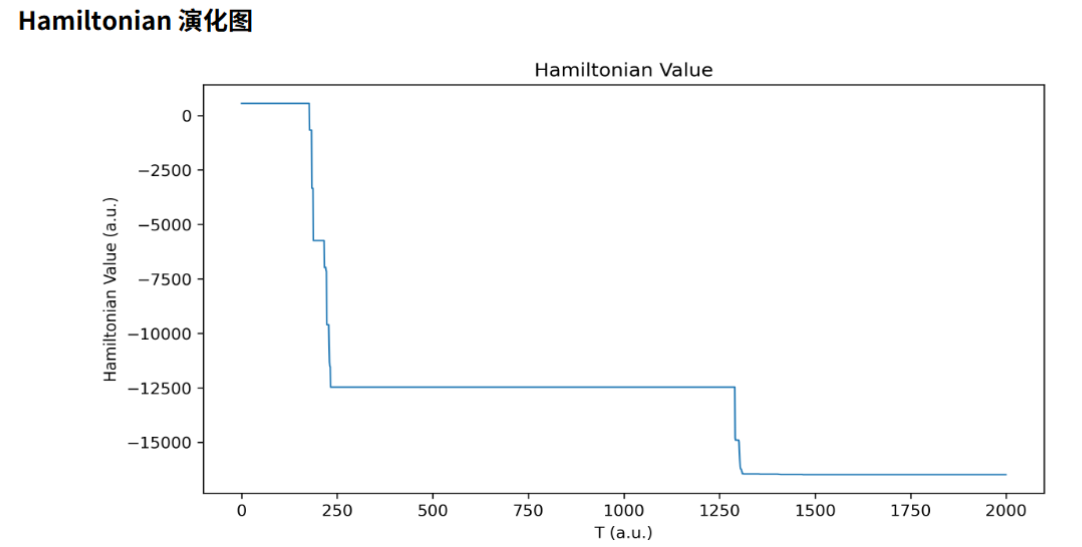
\includegraphics[width=0.8\textwidth]{figures/Q4-hamiltonian.png}
    \caption{Hamiltonian trajectory for Problem~4, showing major drops after slack consolidation and bit trimming; the two highlighted jumps correspond to slack removal (iteration~2) and scenario pruning (iteration~4) according to the solver log.}
    \label{fig:q4_hamiltonian}
\end{figure}

This trajectory confirms that the reduction strategy compresses the dense 7,024-bit energy basin to 435 bits while preserving feasibility, enabling Problem~4 to build a compact QUBO that the Kaiwu hardware can execute.

Collectively, Problems~3 and~4 establish a tangible path from classical UC to hardware-executable quantum approximations.

\section{Strengths and Weaknesses}

\subsection{Strengths of Our Approach}

\begin{description}
\item[Comprehensive Model Integration] Our framework integrates classical optimization with quantum-inspired solvers, as demonstrated by the four sequential problems.

\item[Multi-Constraint Handling] Economic, network, reserve, and contingency constraints are all captured explicitly, yielding realistic schedules.

\item[Scalable Architecture] The modular decomposition from Problems~1 to~4 offers a clear blueprint for adding new constraints or reduction strategies.

\item[Quantum-Classical Comparison] Tables~\ref{tab:q1_meta}--\ref{tab:q3_compare} quantify where quantum methods excel or fall short relative to the classical benchmark.

\item[Practical Assumptions] The assumptions made earlier align with real UC operations, ensuring practical relevance.
\end{description}

\subsection{Weaknesses and Limitations}

\begin{description}
\item[Computational Complexity] The network-constrained model (Problem~2) still requires tens of thousands of simplex iterations despite presolve reductions.

\item[Quantum Hardware Limitations] Current bit counts exceed many devices' capacities, forcing aggressive reduction in Problem~4.

\item[Solution Quality Trade-offs] Binary encodings introduce approximation errors that manifest as residuals in Table~\ref{tab:q3_compare}.

\item[Network Simplifications] We rely on DC power flow and neglect reactive effects, which may be significant under heavy loading.

\item[Deterministic Framework] The workflow assumes perfect forecasts; stochastic or robust variants remain future work.
\end{description}

\subsection{Areas for Improvement}

\begin{itemize}
\item \textbf{Hybrid Solvers}: Combine quantum search for unit commitment patterns with classical dispatch refinement.

\item \textbf{Uncertainty Modeling}: Introduce stochastic reserves or probabilistic outages to better reflect operations.

\item \textbf{Enhanced Reduction}: Automate the scale-reduction heuristics from Problem~4 so that bit budgets are met systematically.
\end{itemize}

%References
\begin{thebibliography}{9}
\bibitem{padhy2004} N.~P.~Padhy, ``Unit commitment -- A bibliographical survey,'' \emph{IEEE Transactions on Power Systems}, vol.~19, no.~3, pp.~1196--1205, 2004.
\bibitem{carrion2006} M.~Carri\'on and J.~M.~Arroyo, ``A computationally efficient mixed-integer linear formulation for the thermal unit commitment problem,'' \emph{IEEE Transactions on Power Systems}, vol.~21, no.~3, pp.~1371--1378, 2006.
\bibitem{lucas2014} A.~Lucas, ``Ising formulations of many NP problems,'' \emph{Frontiers in Physics}, vol.~2, article~5, 2014. doi:10.3389/fphy.2014.00005.
\bibitem{glover2018} F.~Glover, G.~Kochenberger, and Y.~Du, ``Quantum Bridge Analytics I: A tutorial on formulating and using QUBO models,'' \emph{4OR}, vol.~17, pp.~335--371, 2019.
\end{thebibliography}

\newpage
%Appendix

\section{Appendix}

\subsection{Key Implementation Code Snippets}

\subsubsection{Classical UC Model Implementation}
\begin{lstlisting}[language=python,caption={Gurobi Implementation for Classical UC}]
# Classical UC model using Gurobi
model = gp.Model("Classical_UC")

# Decision variables
u = model.addVars(units, time, vtype=GRB.BINARY, name="u")
P = model.addVars(units, time, lb=0, name="P")
y = model.addVars(units, time, vtype=GRB.BINARY, name="y")
z = model.addVars(units, time, vtype=GRB.BINARY, name="z")

# Objective function: minimize total cost
obj = gp.quicksum(a[i]*P[i,t]**2 + b[i]*P[i,t] + c[i]*u[i,t] +
                  SU[i]*y[i,t] + SD[i]*z[i,t]
                  for i in units for t in time)
model.setObjective(obj, GRB.MINIMIZE)

# Power balance constraint
model.addConstrs(gp.quicksum(P[i,t] for i in units) == D[t] for t in time)

# Generation limits
model.addConstrs(P[i,t] >= P_min[i] * u[i,t] for i in units for t in time)
model.addConstrs(P[i,t] <= P_max[i] * u[i,t] for i in units for t in time)

# Start-up/shut-down logic
model.addConstrs(u[i,t] - u[i,t-1] == y[i,t] - z[i,t]
                for i in units for t in time[1:])
model.addConstrs(y[i,t] + z[i,t] <= 1 for i in units for t in time)

# Minimum up/down time constraints
# ... additional constraints implementation
\end{lstlisting}

\subsubsection{QUBO Transformation Code}
\begin{lstlisting}[language=python,caption={QUBO Transformation for UC Problem}]
def uc_to_qubo(uc_problem):
    """Transform UC problem to QUBO format"""
    qubo_matrix = {}
    
    # Objective function terms
    for i in units:
        for t in time:
            # Fuel cost terms
            qubo_matrix[(f"P_{i}_{t}", f"P_{i}_{t}")] = a[i]
            qubo_matrix[(f"u_{i}_{t}", f"u_{i}_{t}")] = c[i]
            # Start-up/shut-down cost terms
            qubo_matrix[(f"y_{i}_{t}", f"y_{i}_{t}")] = SU[i]
            qubo_matrix[(f"z_{i}_{t}", f"z_{i}_{t}")] = SD[i]
    
    # Constraint penalty terms
    for t in time:
        # Power balance constraint
        power_balance_terms = {}
        for i in units:
            power_balance_terms[f"P_{i}_{t}"] = 1
        qubo_matrix = add_penalty_term(qubo_matrix, power_balance_terms, D[t], lambda_pb)
    
    return qubo_matrix
\end{lstlisting}

\end{document}
